\newpage
\section{Architettura}

\subsection{Metodo e Formalismo}
Nell’esposizione dell’architettura dell’applicazione si procederà con un approccio \termine{top-down} descrivendo l’architettura dal generale al particolare. Si procederà quindi alla descrizione dei
\termine{packages} e dei componenti, per poi descrivere nel dettaglio le singole classi, specificando per
ognuna il tipo, l’obiettivo, la funzione, relazioni in ingresso e uscita e i metodi e attributi contenuti. Successivamente si procederà ad elencare i diagrammi di sequenza che descriveranno il funzionamento dell'\termine{SDK} e dell'applicazione. 


\subsection{Informazioni Generali}
Il principio di progettazione che abbiamo addottato è il Common Closure Principale per i seguenti motivi:
\begin{itemize}
\item Suddivisione più logica dei vari package e classi.
\item Aumenta la manutenibilità del codice nel tempo.
\end{itemize}

\subsection{Prodotto software}
Il prodotto che il gruppo \gruppo\ si impone a fare è composto da due parti: \termine{SDK} e \termine{Applicazione}. Per cui verranno prima illustrate i packages dell'\termine{SDK} e poi quelli relativi all'applicazione.

%\begin{figure}[H]
%	\centering
%	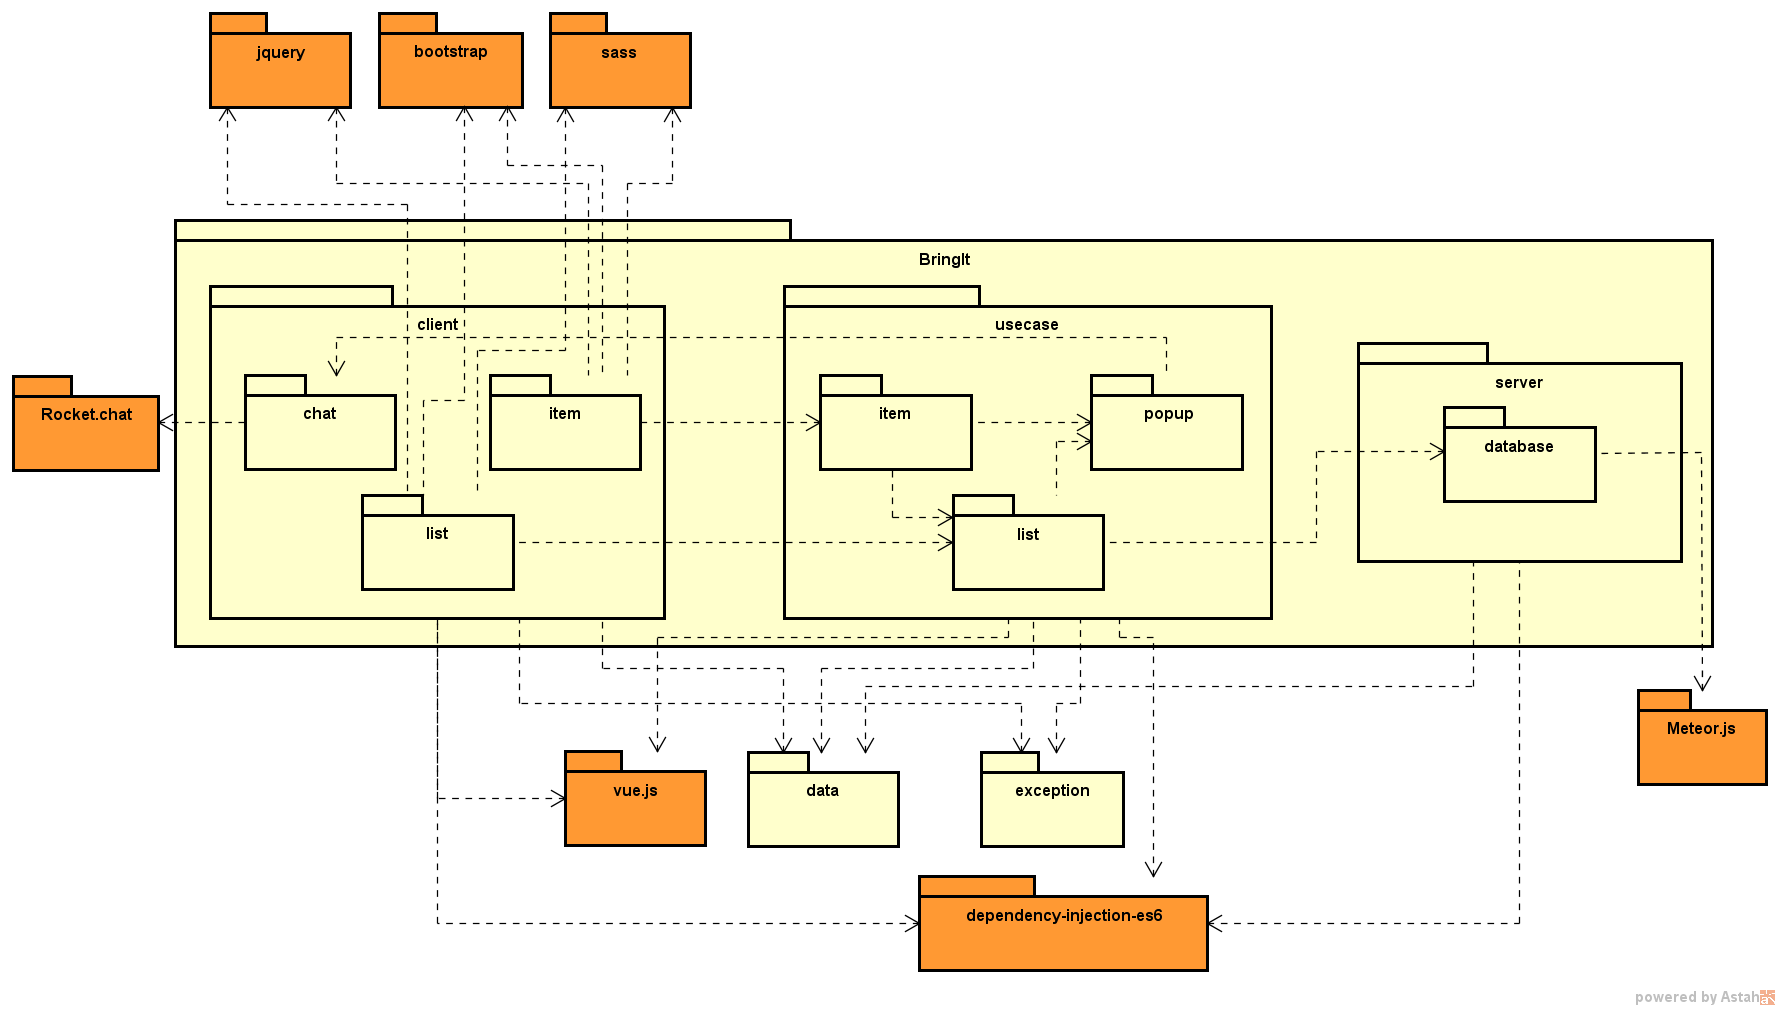
\includegraphics[scale=0.4]{Sezioni/Packages/App/pck_application.png}
%	\caption{Package application}
%\end{figure}


\subsection{SDK}

\subsubsection{Creazione di un widget immagine}

\label{Creazione di un widget immagine}
\begin{figure}[ht]
	\centering
	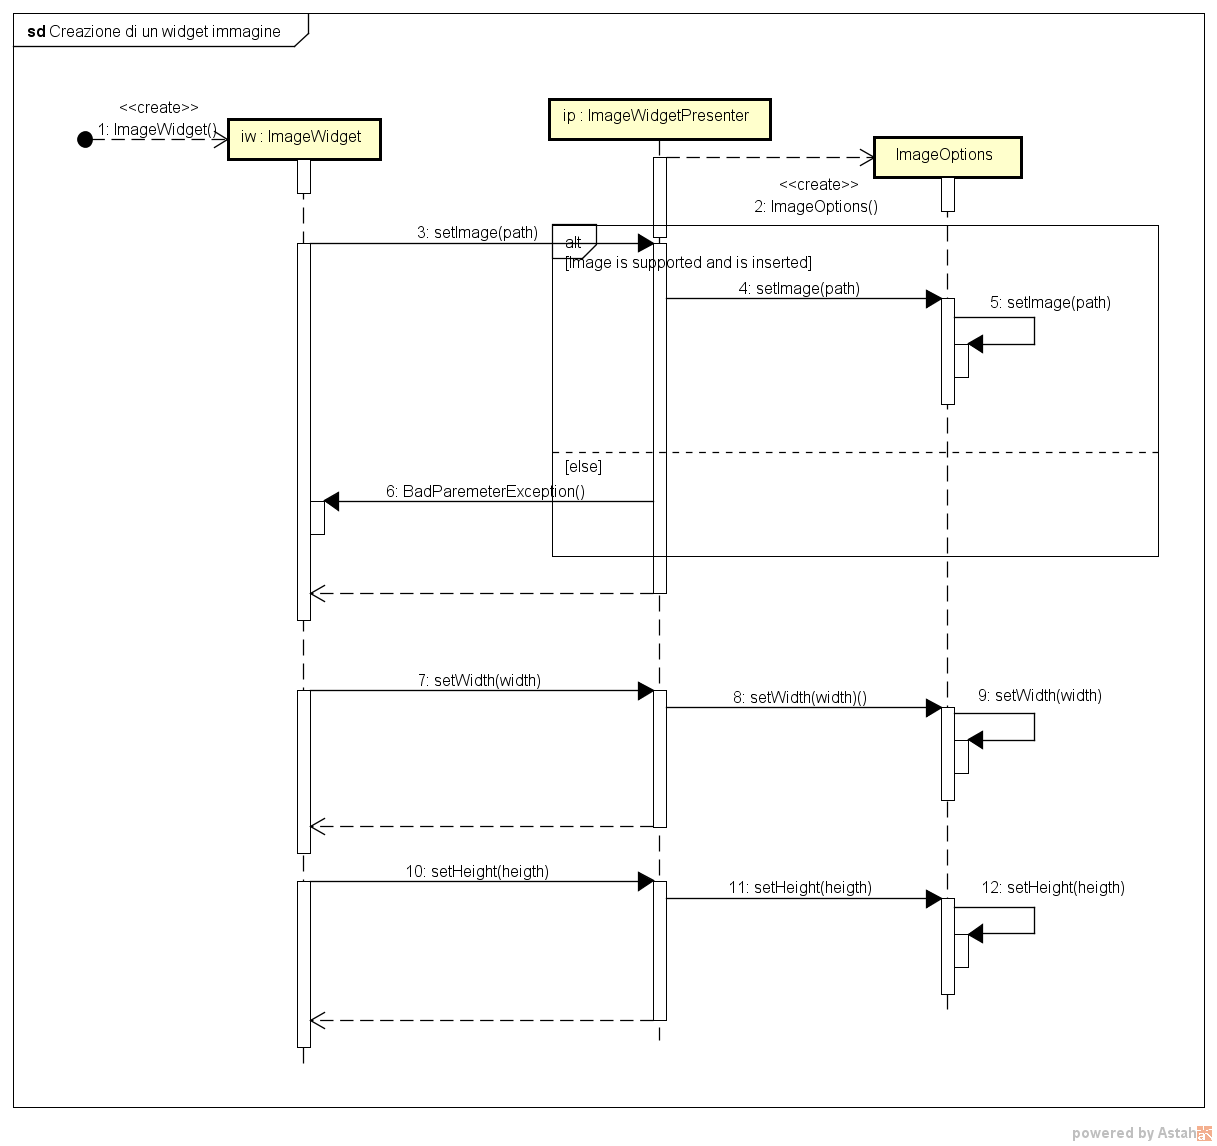
\includegraphics[width=16cm, height=14cm]{Sezioni/Diagrammi/img/Creazione di un widget immagine.png}
	\caption{Creazione di un widget immagine}
\end{figure}

Lo sviluppatore può creare un widget di tipo immagine per aggiungerlo ad una sua ipotetica \termine{bolla}. Durante la costruzione, come si vede dallo schema, vengono invocati tre metodi. Il primo per impostare l'immagine e gli altri due per impostare rispettivamente la larghezza ed altezza di essa. Il tipo delle immagini supportate sono le stesse supportate da \termine{Rocket.Chat} ovvero:
\begin{itemize}
\item .jpeg
\item .gif
\item .png
\item .jpg
\end{itemize}
Se l'immagine inserita non appartiene ad uno di questi formati oppure non viene inserita dallo sviluppatore il metodo \texttt{setText} di \texttt{TextWidgetPresenter} lancerà un'eccezione di tipo \texttt{BadParameterException}. \\
Le frecce di ritorno dall'\texttt{ImageWidgetPresenter} all'\texttt{ImageWidget} sono state inserite poiché il cambiamento dei dati sul \termine{Presenter} ha effetto anche sulla View. La comunicazione tra queste due unità avviene tramite il \termine{framework} \termine{vue.js}. \\
Si noti, infine, che i metodi invocati da \texttt{ImageWidget} vengono chiamati in quest'ordine dal suo costruttore senza parametri. Tali metodi possono anche essere chiamati singolarmente dallo sviluppatore secondo l'ordine che egli preferisce. Queste azioni non verranno ulteriormente descritte poiché ritenute ridondanti.

\newpage

\subsubsection{Creazione di un widget di testo}

\label{Creazione di un widget di testo}
\begin{figure}[H]
	\centering
	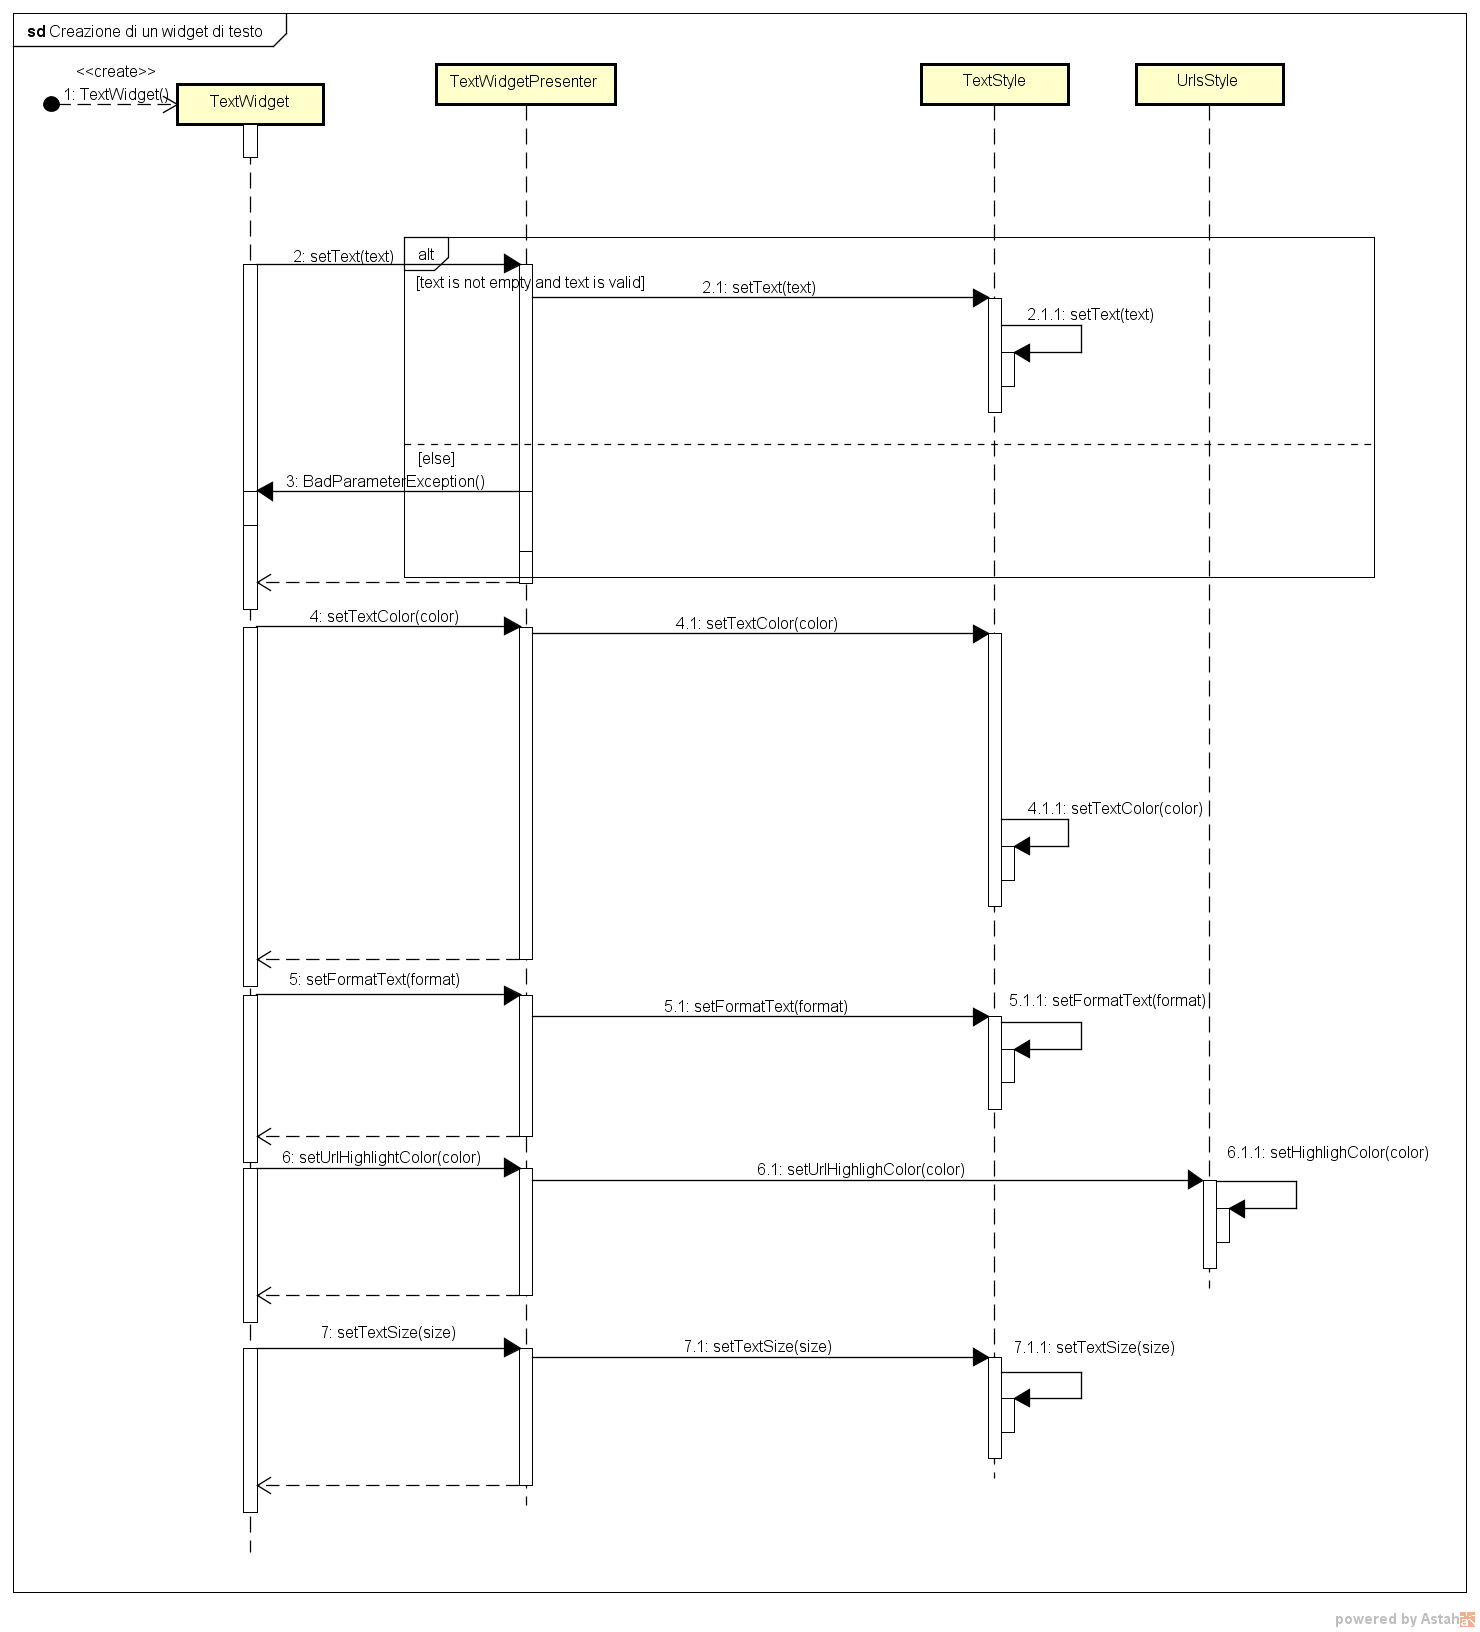
\includegraphics[width=16cm, height=14cm]{Sezioni/Diagrammi/img/Creazione di un widget di testo.png}
	\caption{Creazione di un widget di testo}
\end{figure}

Lo sviluppatore può creare un widget di tipo testo per aggiungerlo ad una sua ipotetica \termine{bolla}. Affinché non si verifichino errori il testo inserito nel widget deve essere valido, ovvero non deve contenere caratteri speciali se non quelli supportati dal tipo di codifica UTF-8 e non deve essere del testo vuoto. Se ciò dovesse capitare il metodo \texttt{setText} di \texttt{TextWidgetPresenter} lancerà un'eccezione di tipo \texttt{BadParameterException}. \\
Le frecce di ritorno dal \texttt{TextWidgetPresenter}  al \texttt{TextWidget} sono state inserite poiché il cambiamento dei dati sul \termine{Presenter} ha effetto anche sulla View. La comunicazione tra queste due unità avviene tramite il \termine{framework} \termine{vue.js}. \\
Si noti, infine, che i metodi invocati da \texttt{TextWidget} vengono chiamati in quest'ordine dal suo costruttore senza parametri. Tali metodi possono anche essere chiamati singolarmente dallo sviluppatore secondo l'ordine che egli preferisce. Queste azioni non verranno ulteriormente descritte poiché ritenute ridondanti.

\newpage

\subsubsection{Creazione di un widget Checklist}

\label{Creazione di un widget Checklist}
\begin{figure}[H]
	\centering
	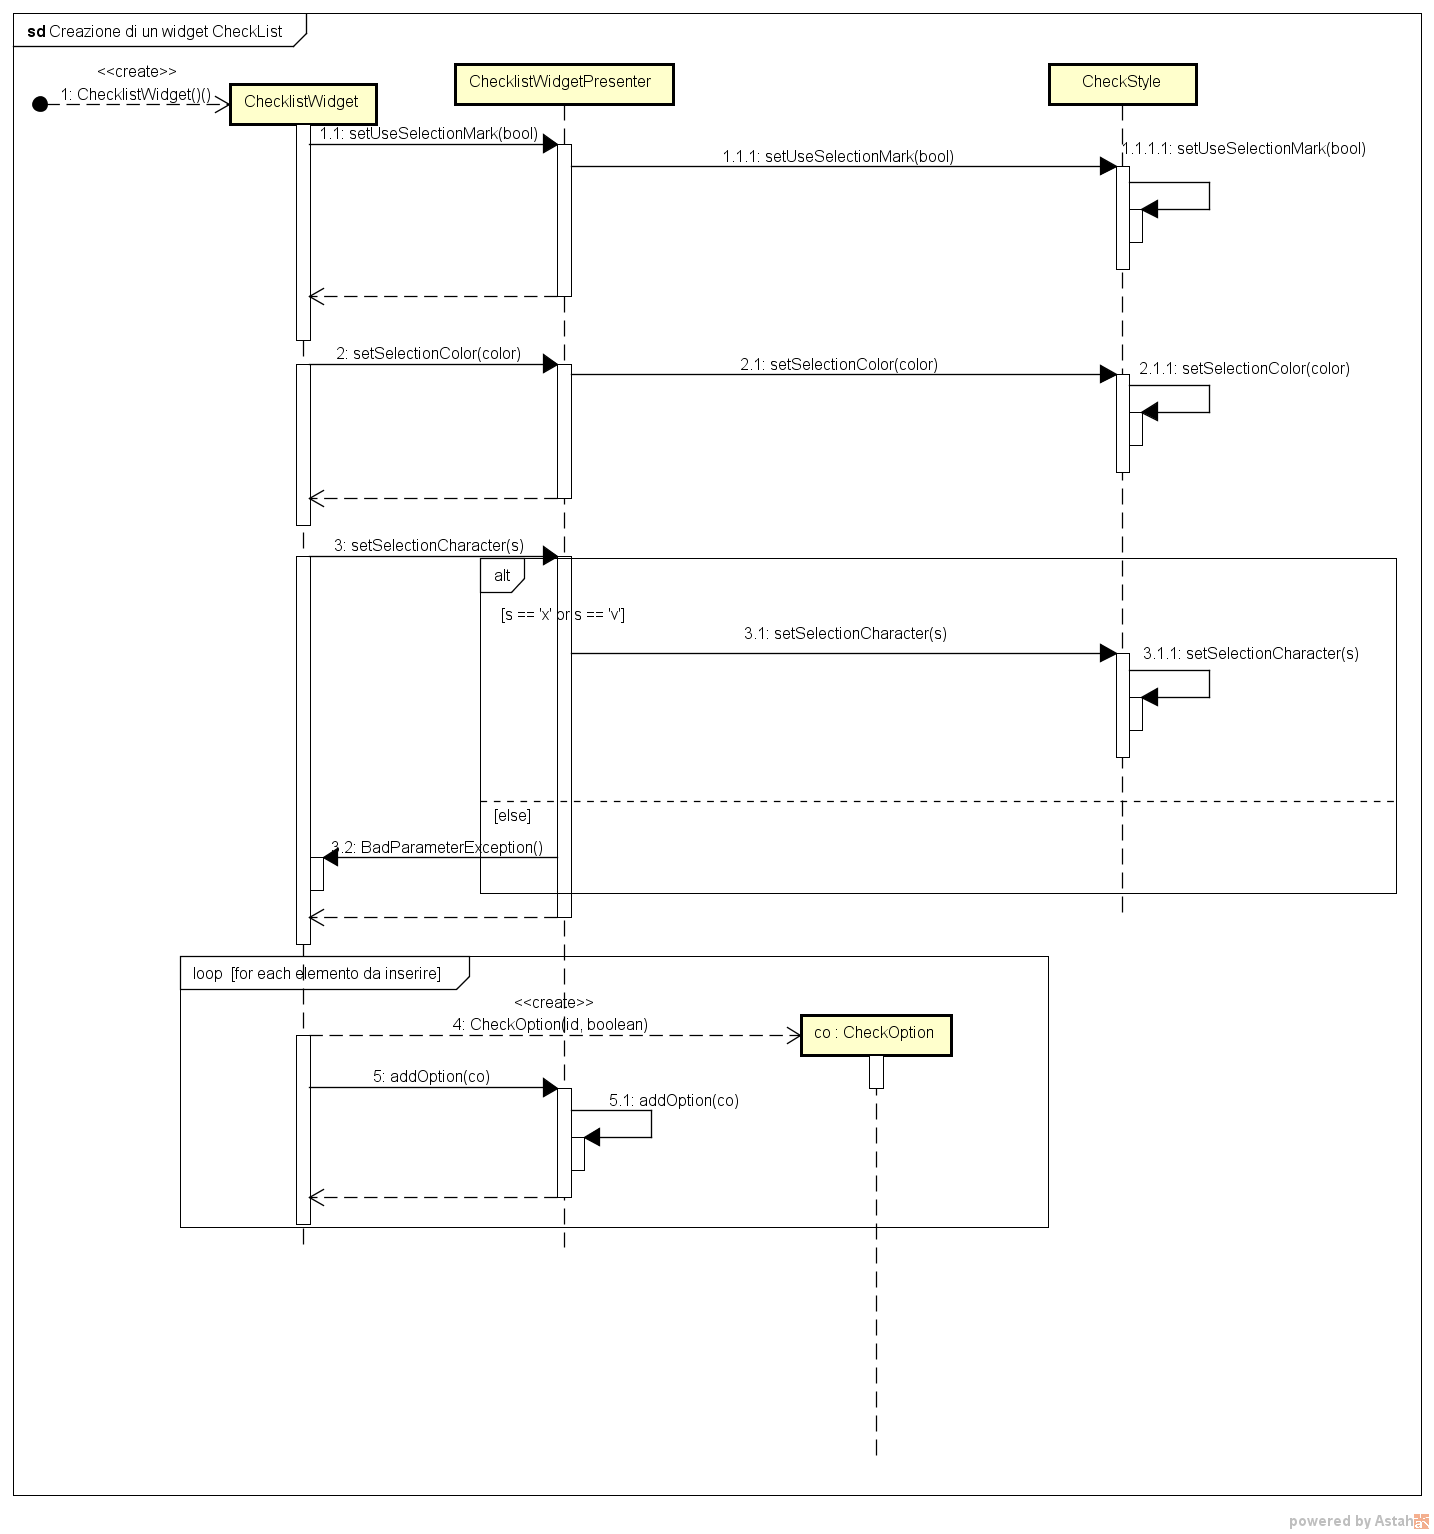
\includegraphics[width=16cm, height=14cm]{Sezioni/Diagrammi/img/Creazione di un widget CheckList.png}
	\caption{Creazione di un widget Checklist}
\end{figure}

Lo sviluppatore può creare un widget di tipo Checklist per aggiungerlo ad una sua ipotetica \termine{bolla}. Affinché non si verifichino errori, quando si usa il metodo \texttt{setSelectionCharacter} deve essere inserito correttamente un carattere per la spunta supportato. Inoltre se il flag \texttt{useSelectionMark} è stato impostato a false allora, indipendentemente dal carattere scelto dalla spunta, verrà usato il colore.\\
Le frecce di ritorno dal \texttt{ChecklistWidgetPresenter}  al \texttt{ChecklistWidget} sono state inserite poiché il cambiamento dei dati sul \termine{Presenter} ha effetto anche sulla View. La comunicazione tra queste due unità avviene tramite il \termine{framework} \termine{vue.js}. \\
Si noti, infine, che i metodi invocati da \texttt{Checklist} vengono chiamati in quest'ordine dal suo costruttore senza parametri. Tali metodi possono anche essere chiamati singolarmente dallo sviluppatore secondo l'ordine che egli preferisce. Queste azioni non verranno ulteriormente descritte poiché ritenute ridondanti.

\newpage

\subsubsection{Aggiungere un messaggio di completamento al widget Checklist}

\label{Aggiungere un messaggio di completamento al widget Checklist}
\begin{figure}[H]
	\centering
	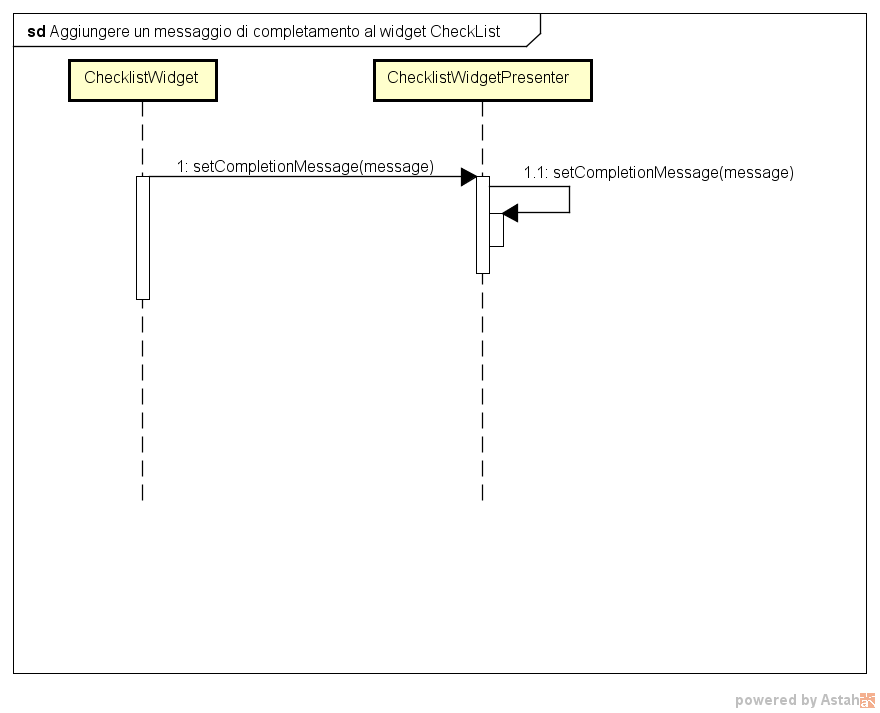
\includegraphics[width=16cm, height=14cm]{Sezioni/Diagrammi/img/Aggiungere un messaggio di completamento al widget Checklist.png}
	\caption{Aggiungere un messaggio di completamento al widget Checklist}
\end{figure}

Lo sviluppatore può aggiungere un messaggio di completamento per il widget Checklist. Questo messaggio verrà visualizzato non appena tutte le entry del widget saranno spuntate, ovvero al lancio dell'evento \texttt{emitOnCompletedList}.

\newpage

\subsubsection{Creazione di un widget bottone}

\label{Creazione di un widget bottone}
\begin{figure}[H]
	\centering
	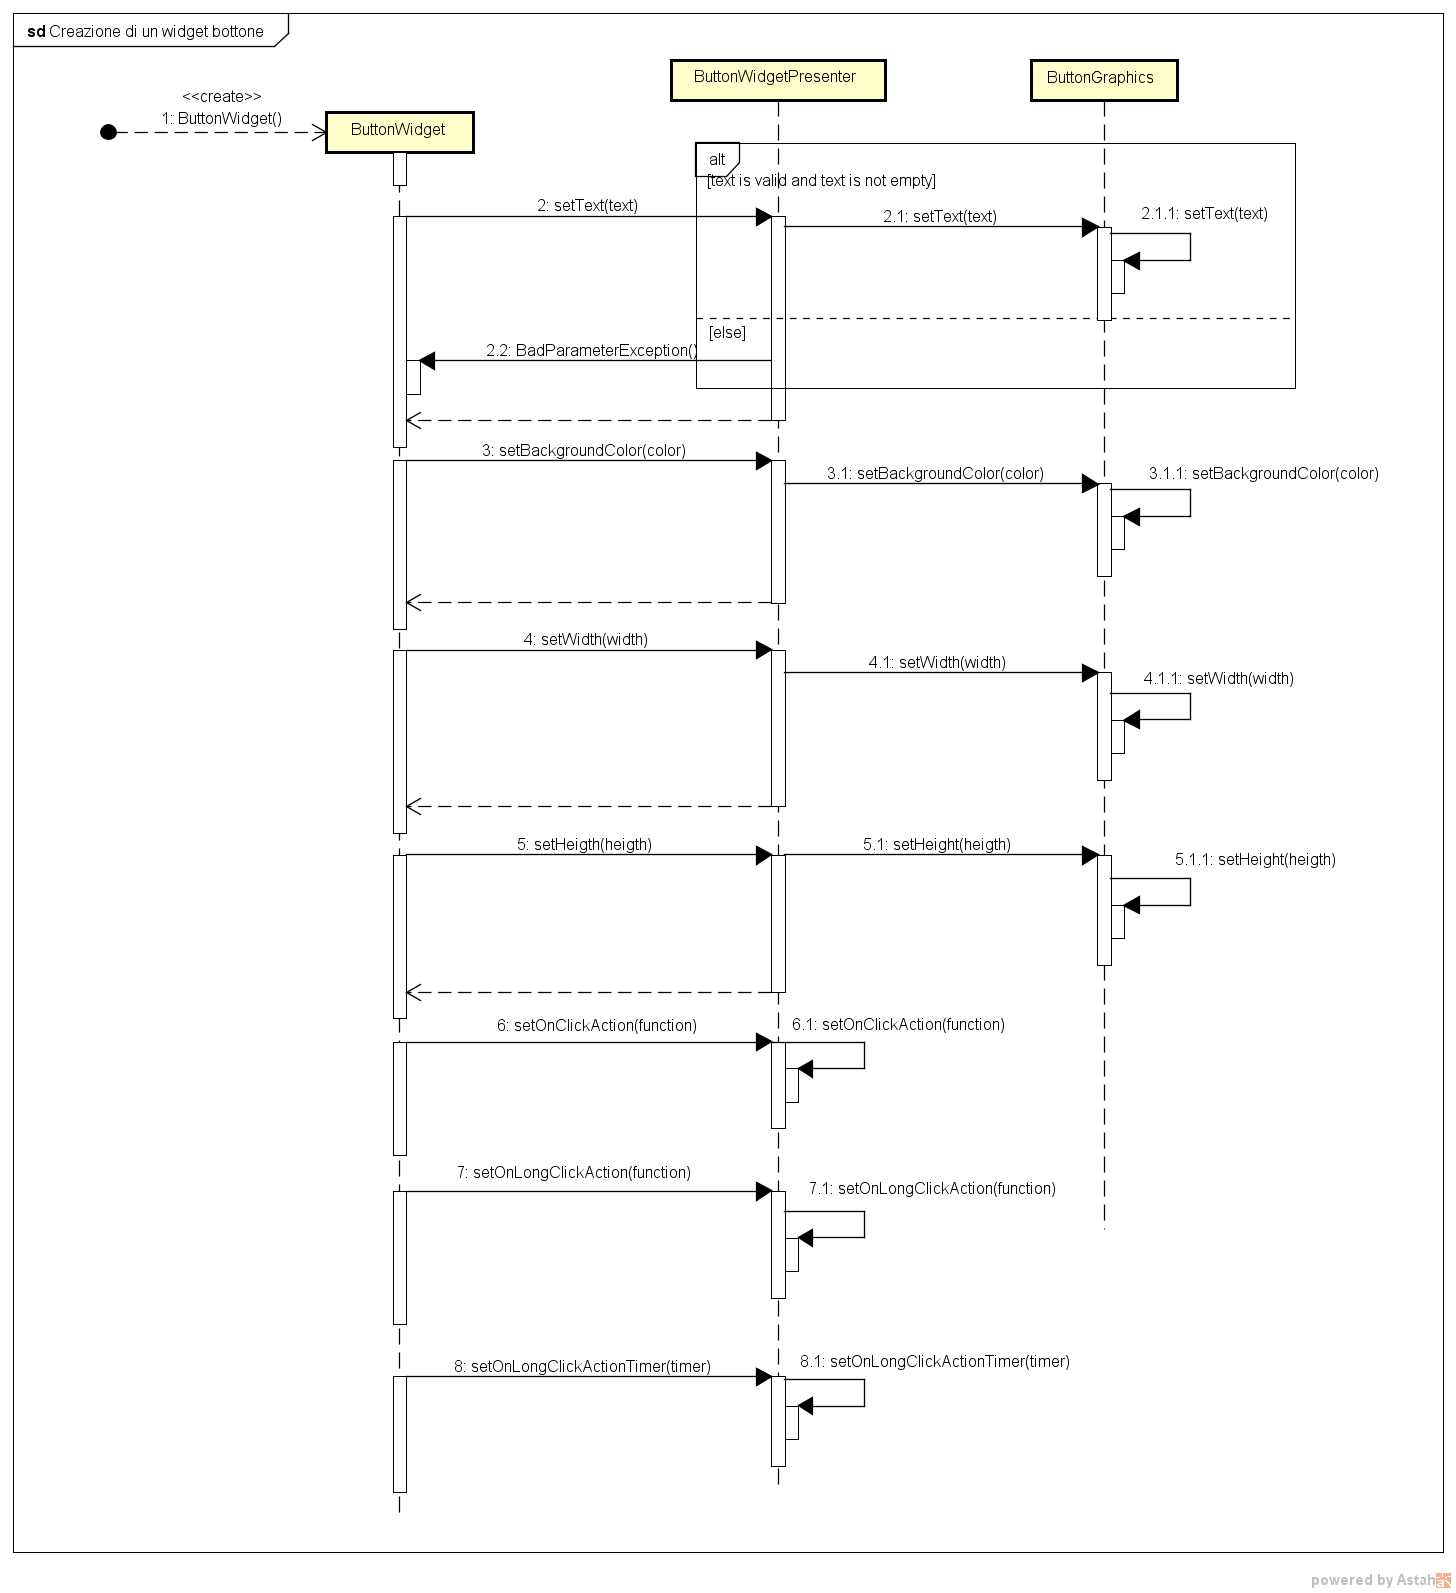
\includegraphics[width=16cm, height=14cm]{Sezioni/Diagrammi/img/Creazione di un widget bottone.png}
	\caption{Creazione di un widget bottone}
\end{figure}

Lo sviluppatore può creare un widget di tipo bottone per aggiungerlo ad una sua ipotetica \termine{bolla}. Se, durante la creazione del widget, il testo non dovesse essere impostato correttamente, il metodo \texttt{setText} di \texttt{ButtonWidgetPresenter} lancerà un'eccezione di tipo \texttt{BadParameterException}. \\
Le frecce di ritorno da \texttt{ButtonWidgetPresenter}  a \texttt{ButtonWidget} sono state inserite poiché il cambiamento dei dati sul \termine{Presenter} ha effetto anche sulla View. La comunicazione tra queste due unità avviene tramite il \termine{framework} \termine{vue.js}. \\
Si noti, infine, che i metodi invocati da \texttt{ButtonWidget} vengono chiamati in quest'ordine dal suo costruttore senza parametri. Tali metodi possono anche essere chiamati singolarmente dallo sviluppatore secondo l'ordine che egli preferisce. Queste azioni non verranno ulteriormente descritte poiché ritenute ridondanti.

\newpage

\subsubsection{Creazione di un listWidget}

\label{Click di un bottone}
\begin{figure}[H]
	\centering
	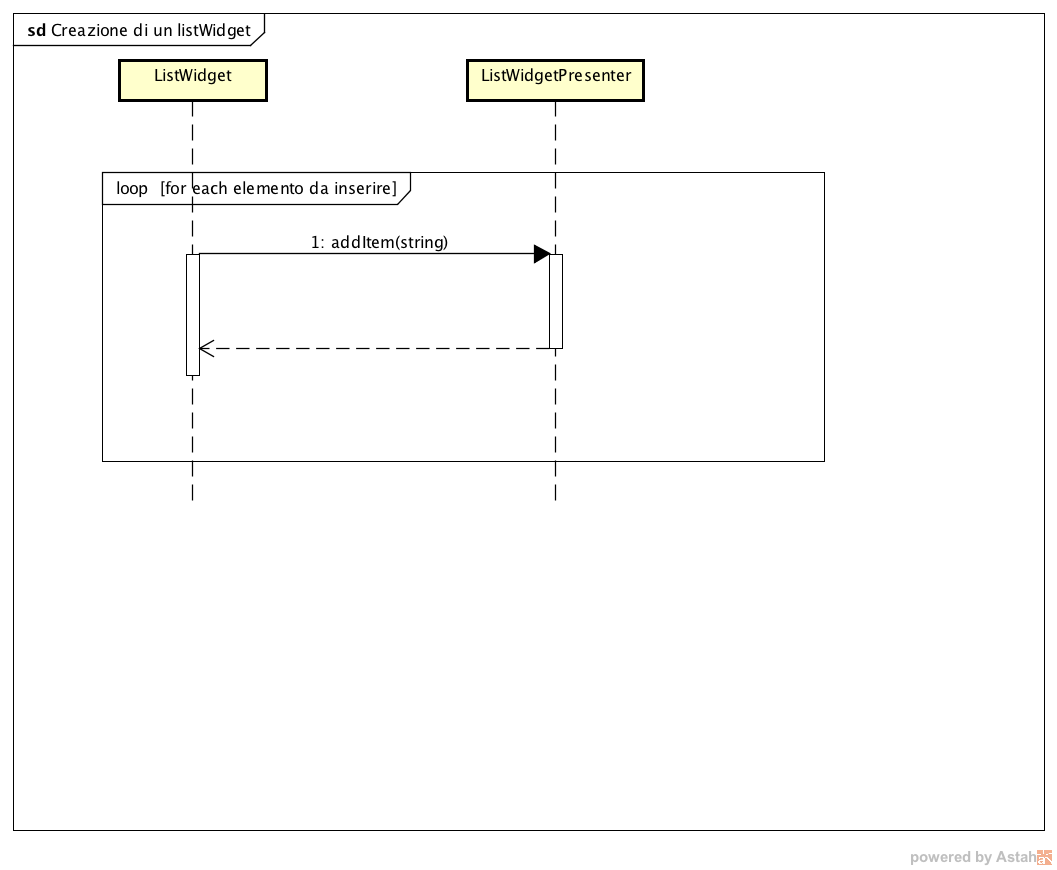
\includegraphics[width=16cm, height=14cm]{Sezioni/Diagrammi/img/Creazione di un listWidget.png}
	\caption{Creazione di un listWidget}
\end{figure}

Lo sviluppatore può creare un widget di tipo lista per aggiungerlo ad una sua ipotetica \termine{bolla}. Ogni elemento aggiunto logicamente dal presenter agisce anche sulla view. Per questo tipo di comunicazione si rimanda al \termine{framework} \termine{vue.js}. \\
L'azione compiuta per creare il widget può essere anche effettuata a posteriori della creazione del widget, questa però, essendo molto simile a quella appena descritta, viene omessa per ridondanza.

\newpage

\subsubsection{Creazione di una bolla aggiungendo un widget checklist}

\label{Creazione di una bolla aggiungendo un widget checklist}
\begin{figure}[H]
	\centering
	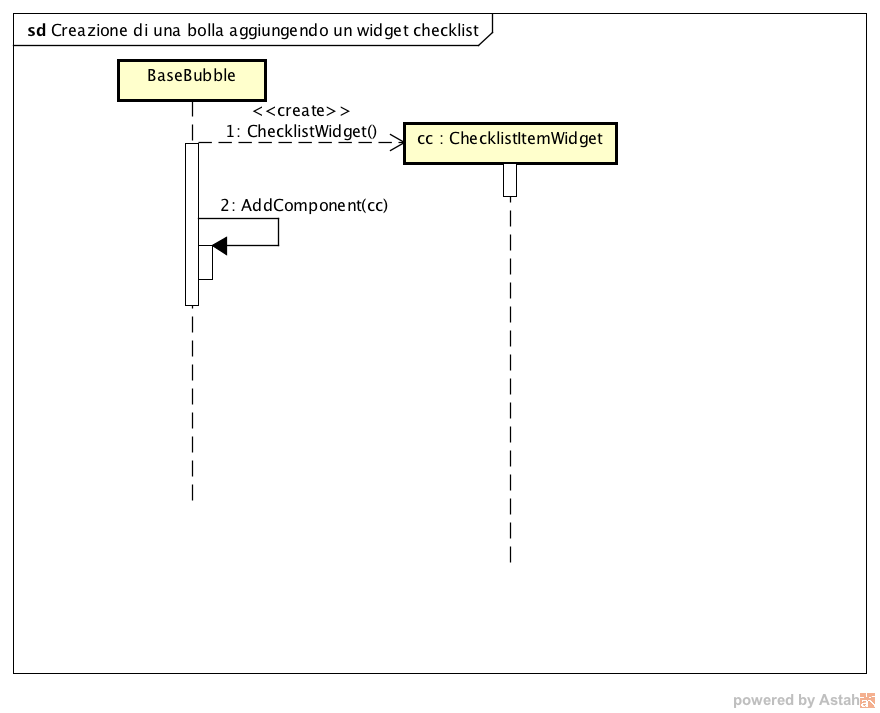
\includegraphics[width=16cm, height=14cm]{Sezioni/Diagrammi/img/Creazione di una bolla aggiungendo un widget checklist.png}
	\caption{Creazione di una bolla aggiungendo un widget checklist}
\end{figure}

Lo sviluppatore può aggiungere un widget alla \termine{bolla} appena creata. L'aggiunta dell'elemento avviene tramite il metodo \texttt{addComponent} che permette l'aggiunta sia di un layout che di un widget. Si noti che l'esempio è fatto con un widget specifico, ovvero il widget checklist, ma ciò vale per qualsiasi widget presente nell'\termine{SDK}. Gli altri esempi simili vengono, per questo motivo, omessi.

\newpage

\subsubsection{Aggiunta ad una bolla di un Layout contenente due widget di testo}

\label{Aggiunta ad una bolla di un Layout contenente due widget di testo}
\begin{figure}[H]
	\centering
	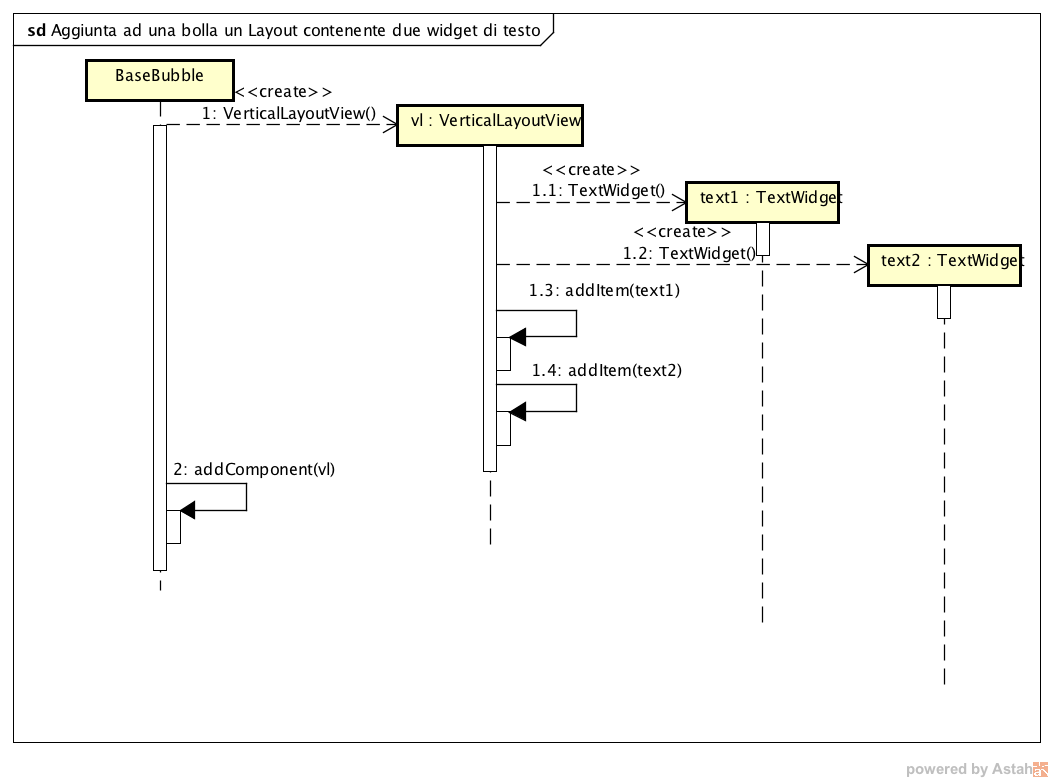
\includegraphics[width=16cm, height=14cm]{Sezioni/Diagrammi/img/Aggiunta ad una bolla un Layout contenente due widget di testo.png}
	\caption{Aggiunta ad una bolla di un Layout contenente due widget di testo}
	
\end{figure}
Lo sviluppatore può aggiungere un layout contenente dei widgets alla \termine{bolla}. Anche questo rappresenta solo un generico esempio di come si possa aggiungere un layout ad una \termine{bolla}. Gli altri esempi simili saranno dunque omessi. 

\newpage

\subsubsection{Creazione di una bolla MarkDownBubble}

\label{Creazione di una bolla MarkDownBubble}
\begin{figure}[H]
	\centering
	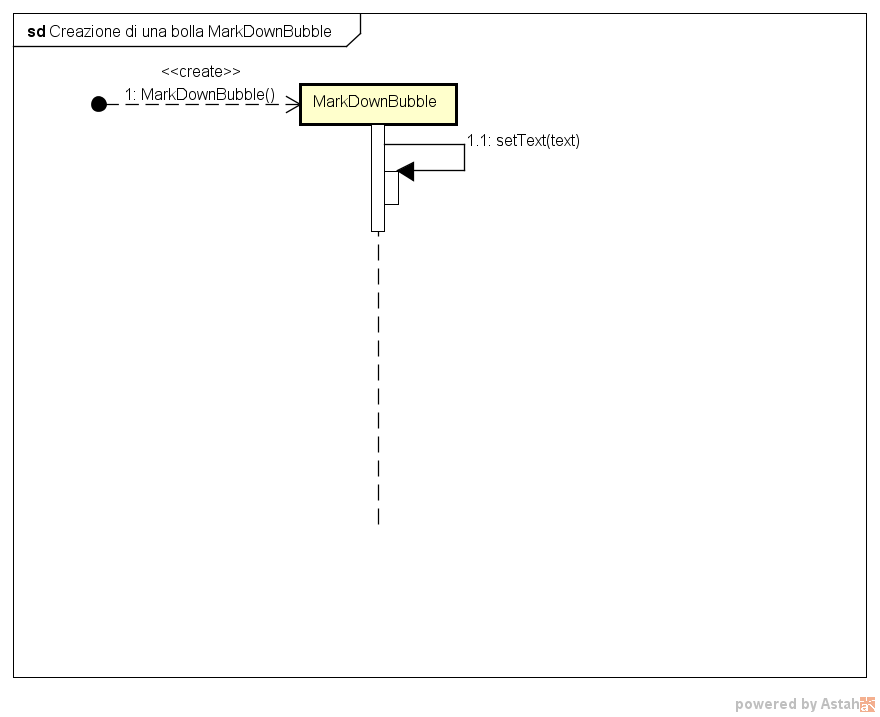
\includegraphics[width=12cm, height=8cm]{Sezioni/Diagrammi/img/Creazione di una bolla MarkDownBubble.png}
	\caption{Creazione di una bolla MarkDownBubble}
	
\end{figure}

Lo sviluppatore può creare una \termine{bolla} MarkDownBubble disponibile nell'\termine{SDK}.

\subsubsection{Creazione di una bolla AlertBubble}

\label{Creazione di una bolla AlertBubble}
\begin{figure}[H]
	\centering
	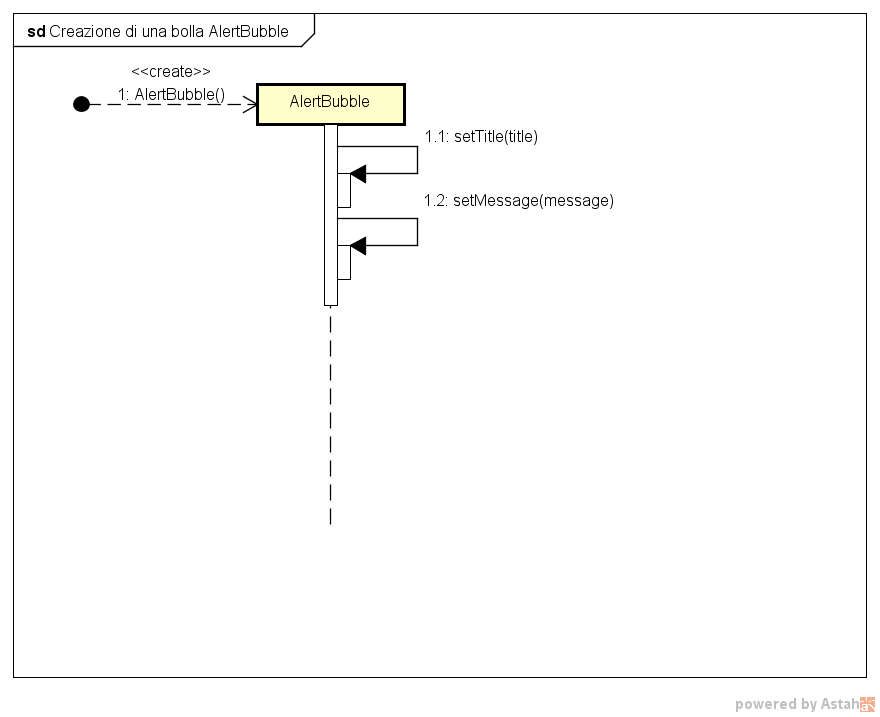
\includegraphics[width=12cm, height=8cm]{Sezioni/Diagrammi/img/Creazione di una bolla AlertBubble.png}
	\caption{Creazione di una bolla AlertBubble}
	
\end{figure}

Lo sviluppatore può creare una \termine{bolla} AlertBubble disponibile nell'\termine{SDK}.

\newpage

\subsubsection{Creazione di una bolla ToDoListBubble}

\label{Creazione di una bolla ToDoListBubble}
\begin{figure}[H]
	\centering
	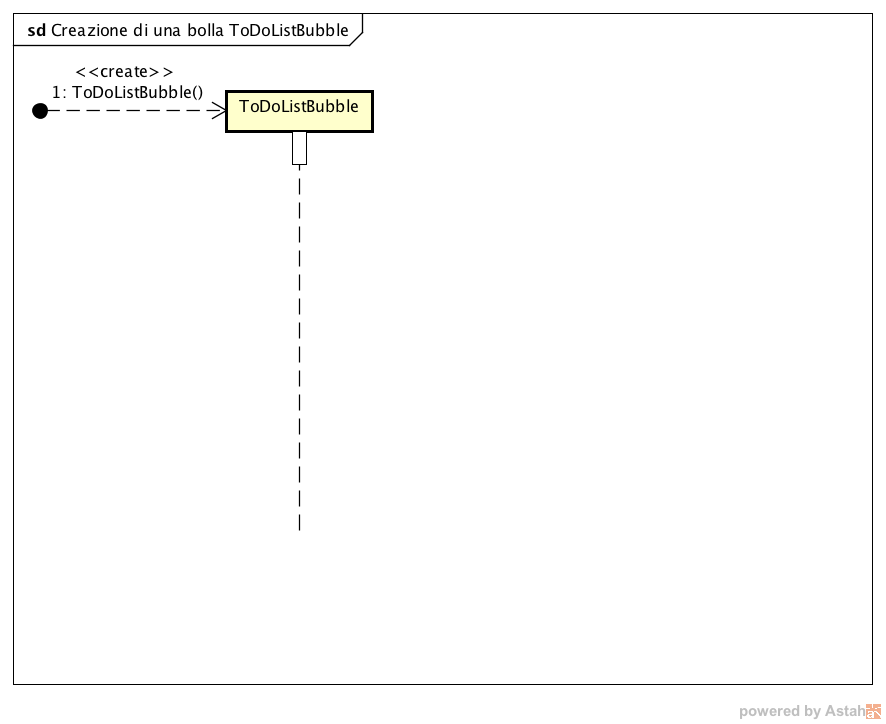
\includegraphics[width=12cm, height=8cm]{Sezioni/Diagrammi/img/Creazione di una bolla ToDoListBubble.png}
	\caption{Creazione di una bolla ToDoListBubble}
	
\end{figure}

Lo sviluppatore può creare una \termine{bolla} ToDoListBubble disponibile nell'\termine{SDK}.



\subsection{Package application}
\label{Package application}
\begin{figure}[H]
	\centering
	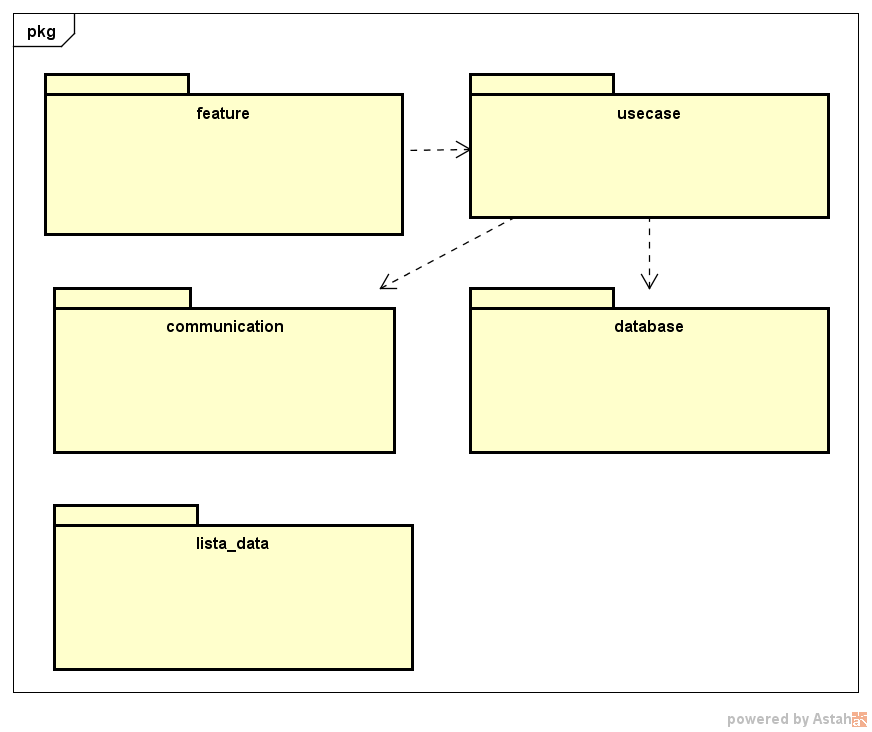
\includegraphics[scale=0.5]{Sezioni/Packages/App/application.png}
	\caption{Package application}
\end{figure}
\begin{itemize}
	\item \textbf{Descrizione}: \termine{Package} contenente tutti i file dell'applicazione demo.
	\item \textbf{Classi e packages contenuti}:
	\begin{itemize}
		\item application::feature: package contenente tutte le feature principali dell'applicazione
		\item application::usecase: package contenente tutti gli usecase dell'applicazione
		\item application::lista\_data: package contenente le classi che modellano i dati dell'applicazione
		\item application::database: package contenente tutte le classi relative ai database
	\end{itemize}
	\item application::communication: package contenente tutte le classi atte a comunicare con la chat
\end{itemize}


\subsubsection{Package application::usecase}
\label{Package application::usecase}
\begin{figure}[H]
	\centering
	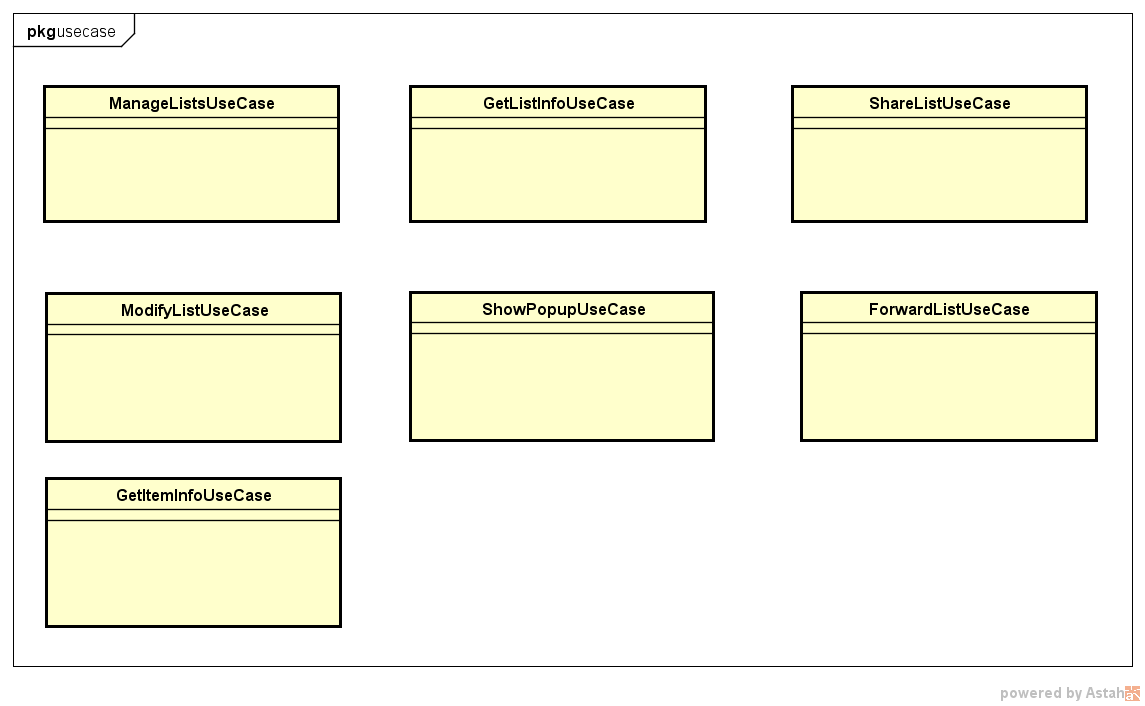
\includegraphics[scale=0.5]{Sezioni/Packages/App/usecase.png}
	\caption{Package application::usecase}
\end{figure}
\begin{itemize}
	\item \textbf{Descrizione}: package contenente tutte le classi che gestiscono la logica dell'applicazione
	\item \textbf{Classi e packages contenuti}:
	\begin{itemize}
	\item application::usecase::ManageListsUseCase: classe che gestisce le modifiche alle liste memorizzate nel database
	\item application::usecase GetListInfoUseCase: classe che recupera i dati di una lista dal database
	\item application::usecase:ModifyListUseCase: classe che permette la modifica di una lista memorizzata all'interno del database
	\item application::usecase ShowPopupUseCase: classe che permette la visualizzazione di finestre modali
	\item application::usecase::GetItemInfoUseCase: classe che permette di recuperare le informazioni di un particolare oggetto in una lista dal database
	\end{itemize}
\end{itemize}

\subsubsection{Package application::lista\_data}
\label{Package application::lista_data}
\begin{figure}[H]
	\centering
	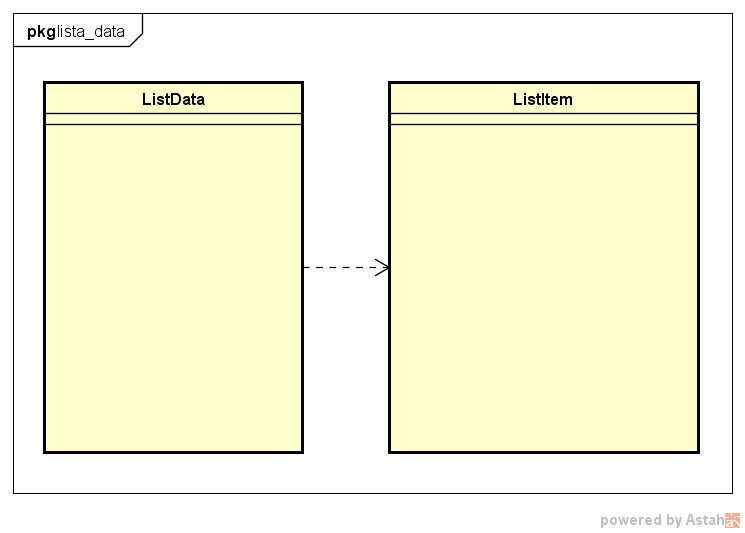
\includegraphics[scale=0.5]{Sezioni/Packages/App/lista_data.png}
	\caption{Package application::lista\_data}
\end{figure}
\begin{itemize}
	\item \textbf{Descrizione}: package contenente tutte le classi che modellano gli oggetti di una lista e di un oggetti di una lista
	\item \textbf{Classi e packages contenuti}:
	\begin{itemize}
	\item application::lista\_data::ListData: classe che modella una lista
	\item application::lista\_data::ListItem: classe che modella un oggetto di una lista
	\end{itemize}
\end{itemize}

\subsubsection{Package application::communication}
\label{Package application::communication}
\begin{figure}[H]
	\centering
	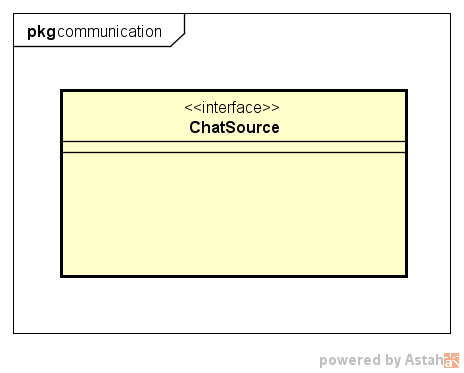
\includegraphics[scale=0.5]{Sezioni/Packages/App/communication.png}
	\caption{Package application::communication}
\end{figure}
\begin{itemize}
	\item \textbf{Descrizione}: package che contiene le classi di comunicazione con l'istanza di Rocket.chat
	\item \textbf{Classi e packages contenuti}:
	\begin{itemize}
	\item application::communication::ChatSource: interfaccia che permette la comunicazione con l'istanza di Rocket.chat
	\end{itemize}
\end{itemize}

\subsubsection{Package application::database}
\label{Package application::database}
\begin{figure}[H]
	\centering
	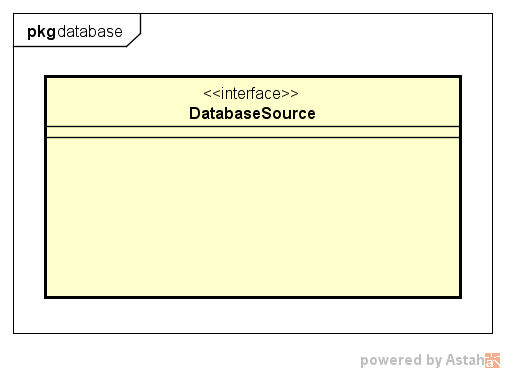
\includegraphics[scale=0.5]{Sezioni/Packages/App/database.png}
	\caption{Package application::database}
\end{figure}
\begin{itemize}
	\item \textbf{Descrizione}: package che contiene le classi per interfacciarsi con il database all'interno del quale sono salvati i dati delle liste
	\item \textbf{Classi e packages contenuti}:
	\begin{itemize}
	\item application::database::DatabaseSource: interfaccia che permette la comunicazione con il database all'interno del quale sono salvati i dati delle varie liste
	\end{itemize}
\end{itemize}

\subsubsection{Package application::feature::add\_item}
\label{Package application::feature::add_item}
\begin{figure}[H]
	\centering
	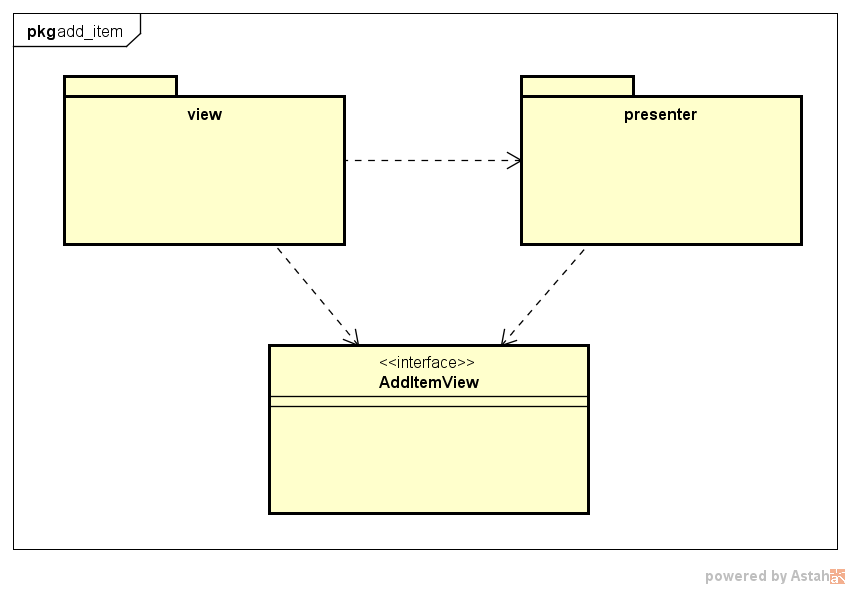
\includegraphics[scale=0.5]{Sezioni/Packages/App/add_item.png}
	\caption{Package application::feature::add\_item}
\end{figure}
\begin{itemize}
	\item \textbf{Descrizione}: package contenente i file relativi alla funzionalità di aggiunta elemento ad una lista
	\item \textbf{Classi e packages contenuti}:
	\begin{itemize}
	\item application::feature::add\_item::view: package contenente la view per l'aggiunta di un elemento
	\item application::feature::add\_item::presenter: package contenente il presenter per la view di aggiunta elemento
	\item application::feature::add\_item::AddItemView: interfaccia che rappresenta la vista di aggiunta oggetto
	\end{itemize}
\end{itemize}

\subsubsection{Package application::feature::add\_item::view}
\label{Package application::feature::add_item::view}
\begin{figure}[H]
	\centering
	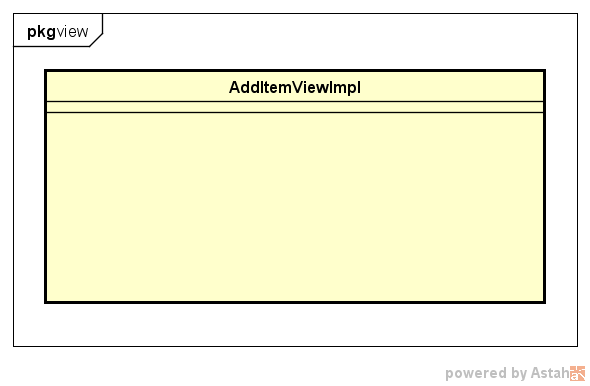
\includegraphics[scale=0.5]{Sezioni/Packages/App/add_item_view.png}
	\caption{Package application::feature::add\_item::view}
\end{figure}
\begin{itemize}
	\item \textbf{Descrizione}: package contenente la view per l'aggiunta di un elemento
	\item \textbf{Classi e packages contenuti}:
	\begin{itemize}
	\item application::feature::add\_item::view::AddItemViewImpl: implementazione dell'interfaccia AddItemView che rappresenta la vista di aggiunta di un oggetto alla lista
	\end{itemize}
\end{itemize}

\subsubsection{Package application::feature::add\_item::presenter}
\label{Package application::feature::add_item::presenter}
\begin{figure}[H]
	\centering
	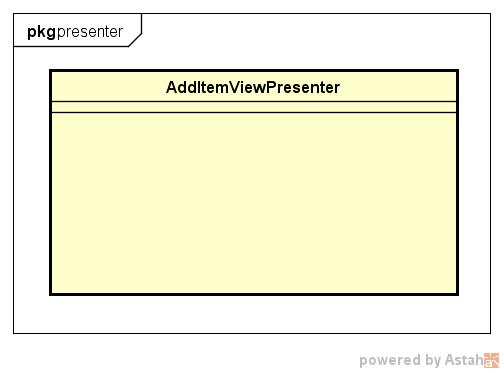
\includegraphics[scale=0.5]{Sezioni/Packages/App/add_item_presenter.png}
	\caption{Package application::feature::add\_item::presenter}
\end{figure}
\begin{itemize}
	\item \textbf{Descrizione}: package contenente il presenter per la vista di aggiunta di un oggetto alla lista
	\item \textbf{Classi e packages contenuti}:
	\begin{itemize}
	\item application::feature::add\_item::presenter::AddItemViewPresenter: presenter per la vista di aggiunta di un oggetto alla lista
	\end{itemize}
\end{itemize}

\subsubsection{Package application::feature::change\_list\_info}
\label{Package application::feature::change_list_info}
\begin{figure}[H]
	\centering
	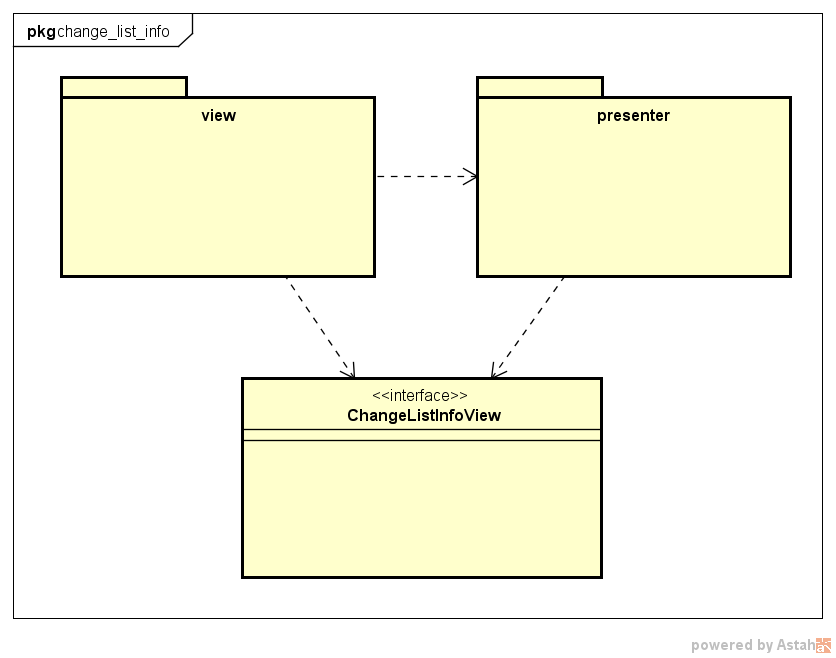
\includegraphics[scale=0.5]{Sezioni/Packages/App/change_list_info.png}
	\caption{Package application::feature::change\_list\_info}
\end{figure}
\begin{itemize}
	\item \textbf{Descrizione}: package contenente i componenti per la funzionalità di modifica informazioni di una lista
	\item \textbf{Classi e packages contenuti}:
	\begin{itemize}
	\item application::feature::change\_list\_info::view: package contenente la vista per la modifica informazioni di una lista
	\item application::feature::change\_list\_info::presenter: package contenente il presenter per la vista di modifica informazioni di una lista
	\item application::feature::change\_list\_info::ChangeListInfoView: interfaccia rappresentante la vista per la modifica informazioni di una lista
	\end{itemize}
\end{itemize}

\subsubsection{Package application::feature::change\_list\_info::view}
\label{Package application::feature::change_list_info::view}
\begin{figure}[H]
	\centering
	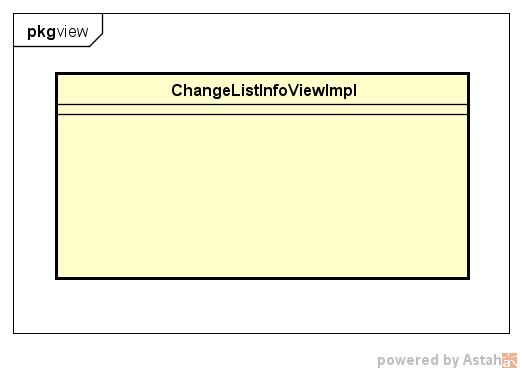
\includegraphics[scale=0.5]{Sezioni/Packages/App/change_list_info_view.png}
	\caption{Package application::feature::change\_list\_info::view}
\end{figure}
\begin{itemize}
	\item \textbf{Descrizione}: package contenente la vista per la funzionalità di modifica informazioni di una lista
	\item \textbf{Classi e packages contenuti}:
	\begin{itemize}
	\item application::feature::change\_list\_info::view::ChangeListInfoViewImpl: implementazione dell'interfaccia che rappresenta la vista per la funzionalità di modifica della informazioni di una lista
	\end{itemize}
\end{itemize}

\subsubsection{Package application::feature::change\_list\_info::presenter}
\label{Package application::feature::change_list_info::presenter}
\begin{figure}[H]
	\centering
	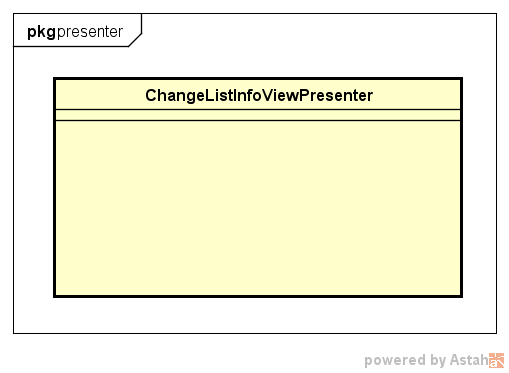
\includegraphics[scale=0.5]{Sezioni/Packages/App/change_list_info_presenter.png}
	\caption{Package application::feature::change\_list\_info::presenter}
\end{figure}
\begin{itemize}
	\item \textbf{Descrizione}: package contenente il presenter per la vista di modifica informazioni di una lista
	\item \textbf{Classi e packages contenuti}:
	\begin{itemize}
	\item application::feature::change\_list\_info::presenter::ChangeListInfoViewPresenter: classe che rappresenta il presenter per la vista di modifica dei dati di una lista
	\end{itemize}
\end{itemize}


\subsubsection{Package application::feature::create\_list}
\label{Package application::feature::create_list}
\begin{figure}[H]
	\centering
	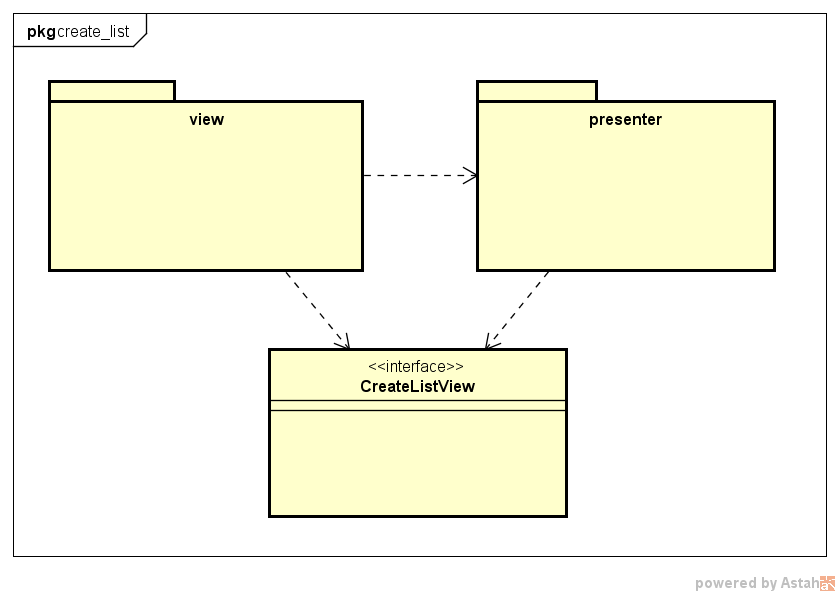
\includegraphics[scale=0.5]{Sezioni/Packages/App/create_list.png}
	\caption{Package application::feature::create\_list}
\end{figure}
\begin{itemize}
	\item \textbf{Descrizione}: package contenente i componenti per la funzionalità di creazione di una lista
	\item \textbf{Classi e packages contenuti}:
	\begin{itemize}
	\item application::feature::create\_list::view: package contenente la vista per la creazione di una lista
	\item application::feature::create\_list::presenter: package contenente il presenter per la vista di creazione di una lista
	\item application::feature::create\_list::CreateListView: interfaccia rappresentante la vista per la creazione di una lista
	\end{itemize}
\end{itemize}

\subsubsection{Package application::feature::create\_list::view}
\label{Package application::feature::create_list::view}
\begin{figure}[H]
	\centering
	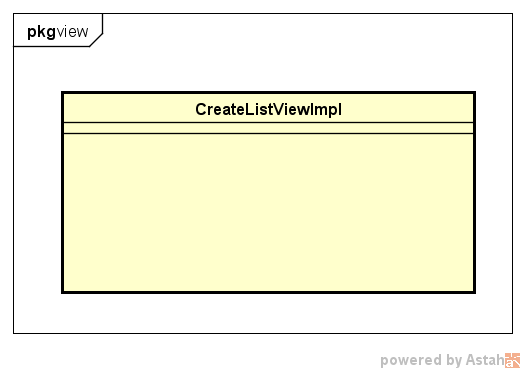
\includegraphics[scale=0.5]{Sezioni/Packages/App/create_list_view.png}
	\caption{Package application::feature::create\_list::view}
\end{figure}
\begin{itemize}
	\item \textbf{Descrizione}: package contenente la vista per la funzionalità di creazione di una lista
	\item \textbf{Classi e packages contenuti}:
	\begin{itemize}
	\item application::feature::create\_list::view::CreateListViewImpl: implementazione dell'interfaccia che rappresenta la vista per la funzionalità di creazione di una lista
	\end{itemize}
\end{itemize}

\subsubsection{Package application::feature::create\_list::presenter}
\label{Package application::feature::create_list::presenter}
\begin{figure}[H]
	\centering
	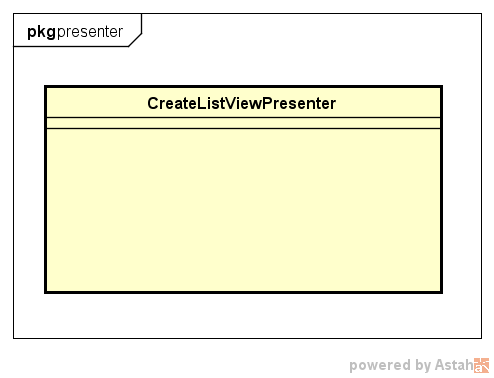
\includegraphics[scale=0.5]{Sezioni/Packages/App/create_list_presenter.png}
	\caption{Package application::feature::create\_list::presenter}
\end{figure}
\begin{itemize}
	\item \textbf{Descrizione}: package contenente il presenter per la vista di creazione di una lista
	\item \textbf{Classi e packages contenuti}:
	\begin{itemize}
	\item application::feature::create\_list::presenter::CreateListViewPresenter: classe che rappresenta il presenter per la vista di creazione di una lista
	\end{itemize}
\end{itemize}

\subsubsection{Package application::feature::forward}
\label{Package application::feature::forward}
\begin{figure}[H]
	\centering
	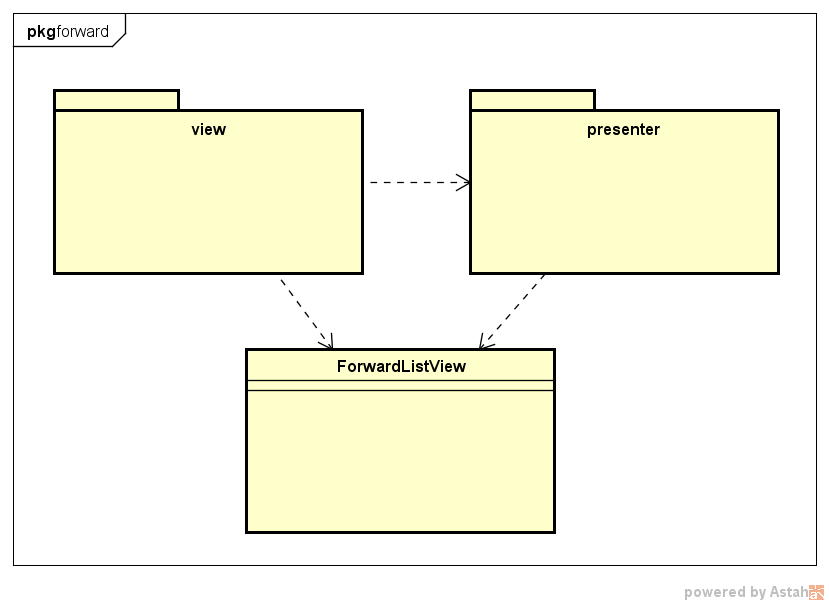
\includegraphics[scale=0.5]{Sezioni/Packages/App/forward.png}
	\caption{Package application::feature::forward}
\end{figure}
\begin{itemize}
	\item \textbf{Descrizione}: package contenente i componenti per la funzionalità di inoltro di una lista
	\item \textbf{Classi e packages contenuti}:
	\begin{itemize}
	\item application::feature::forward::view: package contenente la vista per la inoltro di una lista
	\item application::feature::forward::presenter: package contenente il presenter per la vista di inoltro di una lista
	\item application::feature::forward::ForwardListView: interfaccia rappresentante la vista per la funzionalità inoltro di una lista
	\end{itemize}
\end{itemize}

\subsubsection{Package application::feature::forward::view}
\label{Package application::feature::forward::view}
\begin{figure}[H]
	\centering
	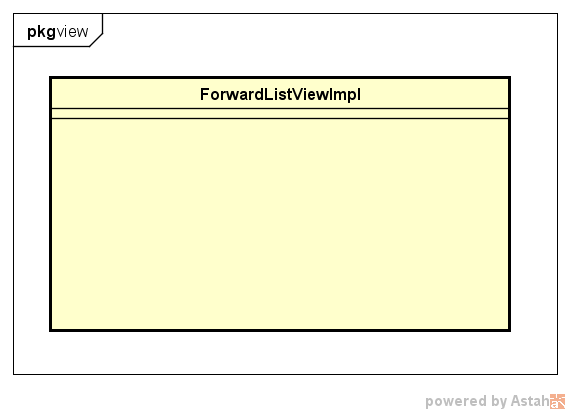
\includegraphics[scale=0.5]{Sezioni/Packages/App/forward_view.png}
	\caption{Package application::feature::forward::view}
\end{figure}
\begin{itemize}
	\item \textbf{Descrizione}: package contenente la vista per la funzionalità di inoltro di una lista
	\item \textbf{Classi e packages contenuti}:
	\begin{itemize}
	\item application::feature::forward::view::ForwardListViewImpl: implementazione dell'interfaccia che rappresenta la vista per la funzionalità di inoltro di una lista
	\end{itemize}
\end{itemize}

\subsubsection{Package application::feature::forward::presenter}
\label{Package application::feature::forward::presenter}
\begin{figure}[H]
	\centering
	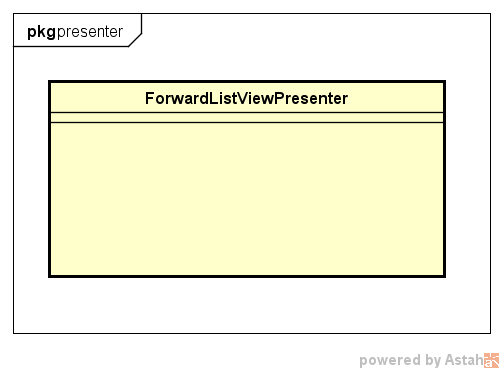
\includegraphics[scale=0.5]{Sezioni/Packages/App/forward_presenter.png}
	\caption{Package application::feature::forward::presenter}
\end{figure}
\begin{itemize}
	\item \textbf{Descrizione}: package contenente il presenter per la vista di inoltro di una lista
	\item \textbf{Classi e packages contenuti}:
	\begin{itemize}
	\item application::feature::forward::presenter::ForwardListViewPresenter: classe che rappresenta il presenter per la vista di inoltro di una lista
	\end{itemize}
\end{itemize}

\subsubsection{Package application::feature::input\_item\_info}
\label{Package application::feature::input_item_info}
\begin{figure}[H]
	\centering
	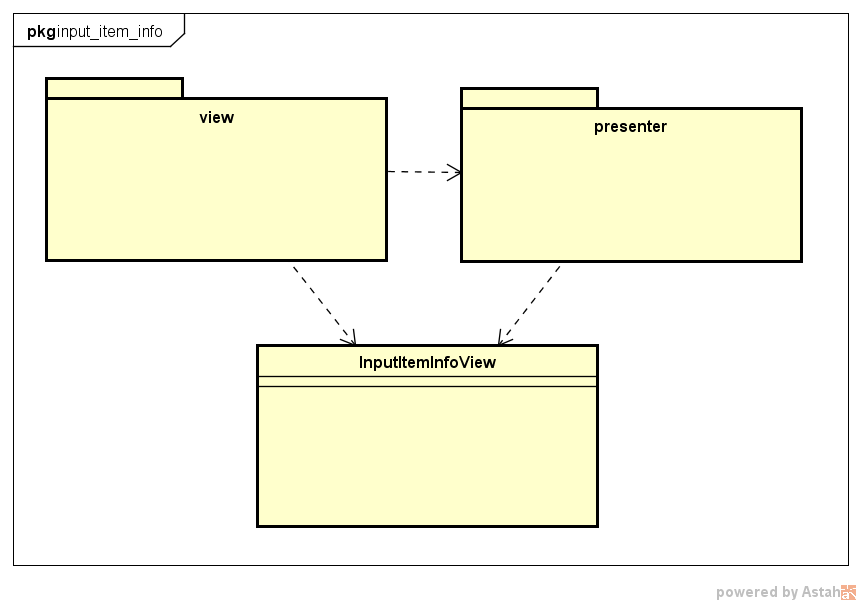
\includegraphics[scale=0.5]{Sezioni/Packages/App/input_item_info.png}
	\caption{Package application::feature::input\_item\_info}
\end{figure}
\begin{itemize}
	\item \textbf{Descrizione}: package contenente i componenti per la funzionalità di inserimento dati di un oggetto della lista
	\item \textbf{Classi e packages contenuti}:
	\begin{itemize}
	\item application::feature::input\_item\_info::view: package contenente la vista per la inserimento dati di un oggetto della lista
	\item application::feature::input\_item\_info::presenter: package contenente il presenter per la vista di inserimento dati di un oggetto della lista
	\item application::feature::input\_item\_info::InputItemInfoView: interfaccia rappresentante la vista per la funzionalità inserimento dati di un oggetto della lista
	\end{itemize}
\end{itemize}

\subsubsection{Package application::feature::input\_item\_info::view}
\label{Package application::feature::input_item_info::view}
\begin{figure}[H]
	\centering
	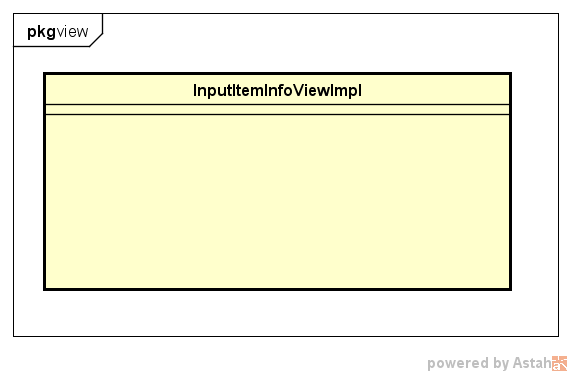
\includegraphics[scale=0.5]{Sezioni/Packages/App/input_item_info_view.png}
	\caption{Package application::feature::input\_item\_info::view}
\end{figure}
\begin{itemize}
	\item \textbf{Descrizione}: package contenente la vista per la funzionalità di inserimento dati di un oggetto della lista
	\item \textbf{Classi e packages contenuti}:
	\begin{itemize}
	\item application::feature::input\_item\_info::view::InputItemInfoViewImpl: implementazione dell'interfaccia che rappresenta la vista per la funzionalità di inserimento dati di un oggetto della lista
	\end{itemize}
\end{itemize}

\subsubsection{Package application::feature::input\_item\_info::presenter}
\label{Package application::feature::input_item_info::presenter}
\begin{figure}[H]
	\centering
	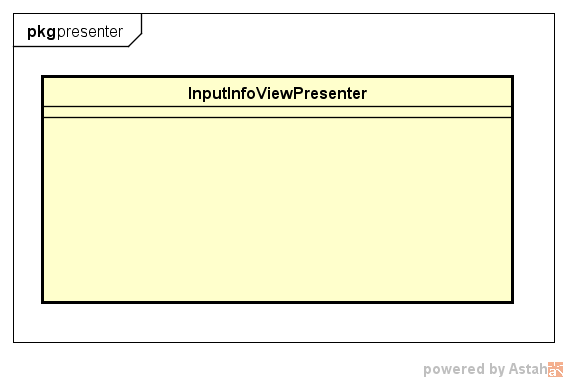
\includegraphics[scale=0.5]{Sezioni/Packages/App/input_item_info_presenter.png}
	\caption{Package application::feature::input\_item\_info::presenter}
\end{figure}
\begin{itemize}
	\item \textbf{Descrizione}: package contenente il presenter per la vista di inserimento dati di un oggetto della lista
	\item \textbf{Classi e packages contenuti}:
	\begin{itemize}
	\item application::feature::input\_item\_info::presenter::InputItemInfoViewPresenter: classe che rappresenta il presenter per la vista di inserimento dati di un oggetto della lista
	\end{itemize}
\end{itemize}


\subsubsection{Package application::feature::input\_list\_info}
\label{Package application::feature::input_list_info}
\begin{figure}[H]
	\centering
	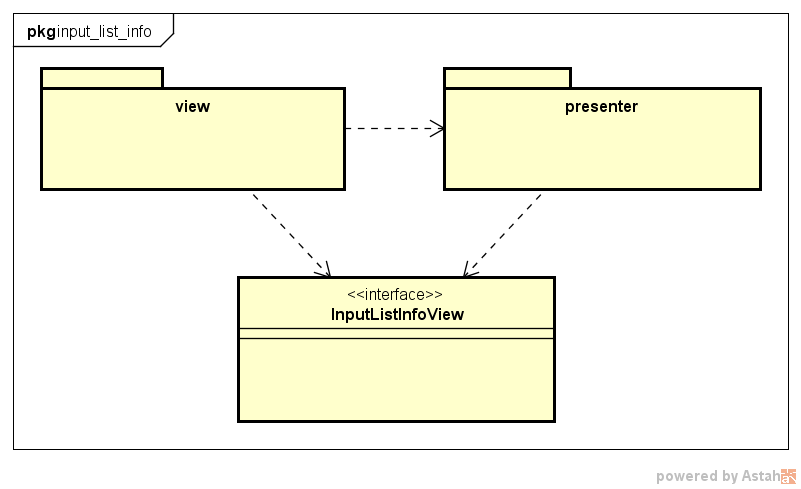
\includegraphics[scale=0.5]{Sezioni/Packages/App/input_list_info.png}
	\caption{Package application::feature::input\_list\_info}
\end{figure}
\begin{itemize}
	\item \textbf{Descrizione}: package contenente i componenti per la funzionalità di inserimento dati di una lista
	\item \textbf{Classi e packages contenuti}:
	\begin{itemize}
	\item application::feature::input\_list\_info::view: package contenente la vista per la inserimento dati di una lista
	\item application::feature::input\_list\_info::presenter: package contenente il presenter per la vista di inserimento dati di una lista
	\item application::feature::input\_list\_info::InputListInfoView: interfaccia rappresentante la vista per la funzionalità inserimento dati di una lista
	\end{itemize}
\end{itemize}

\subsubsection{Package application::feature::input\_list\_info::view}
\label{Package application::feature::input_list_info::view}
\begin{figure}[H]
	\centering
	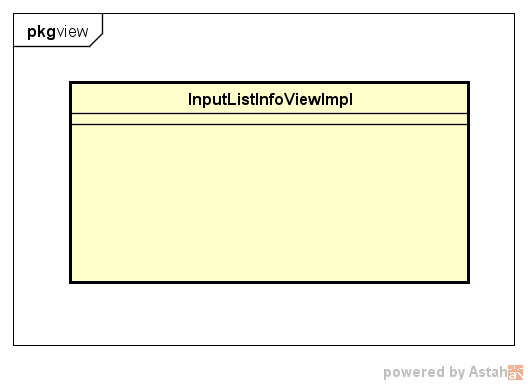
\includegraphics[scale=0.5]{Sezioni/Packages/App/input_list_info_view.png}
	\caption{Package application::feature::input\_list\_info::view}
\end{figure}
\begin{itemize}
	\item \textbf{Descrizione}: package contenente la vista per la funzionalità di inserimento dati di una lista
	\item \textbf{Classi e packages contenuti}:
	\begin{itemize}
	\item application::feature::input\_list\_info::view::InputListInfoViewImpl: implementazione dell'interfaccia che rappresenta la vista per la funzionalità di inserimento dati di una lista
	\end{itemize}
\end{itemize}

\subsubsection{Package application::feature::input\_list\_info::presenter}
\label{Package application::feature::input_list_info::presenter}
\begin{figure}[H]
	\centering
	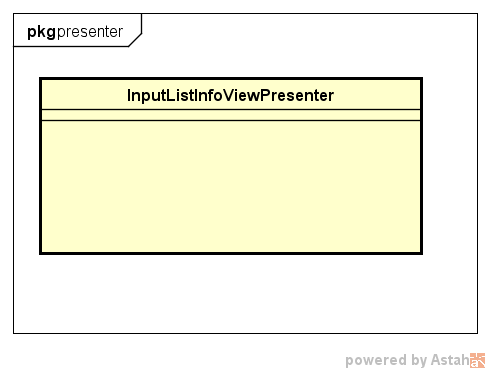
\includegraphics[scale=0.5]{Sezioni/Packages/App/input_list_info_presenter.png}
	\caption{Package application::feature::input\_list\_info::presenter}
\end{figure}
\begin{itemize}
	\item \textbf{Descrizione}: package contenente il presenter per la vista di inserimento dati di una lista
	\item \textbf{Classi e packages contenuti}:
	\begin{itemize}
	\item application::feature::input\_list\_info::presenter::InputListInfoViewPresenter: classe che rappresenta il presenter per la vista di inserimento dati di una lista
	\end{itemize}
\end{itemize}


\subsubsection{Package application::feature::modify\_item}
\label{Package application::feature::modify_item}
\begin{figure}[H]
	\centering
	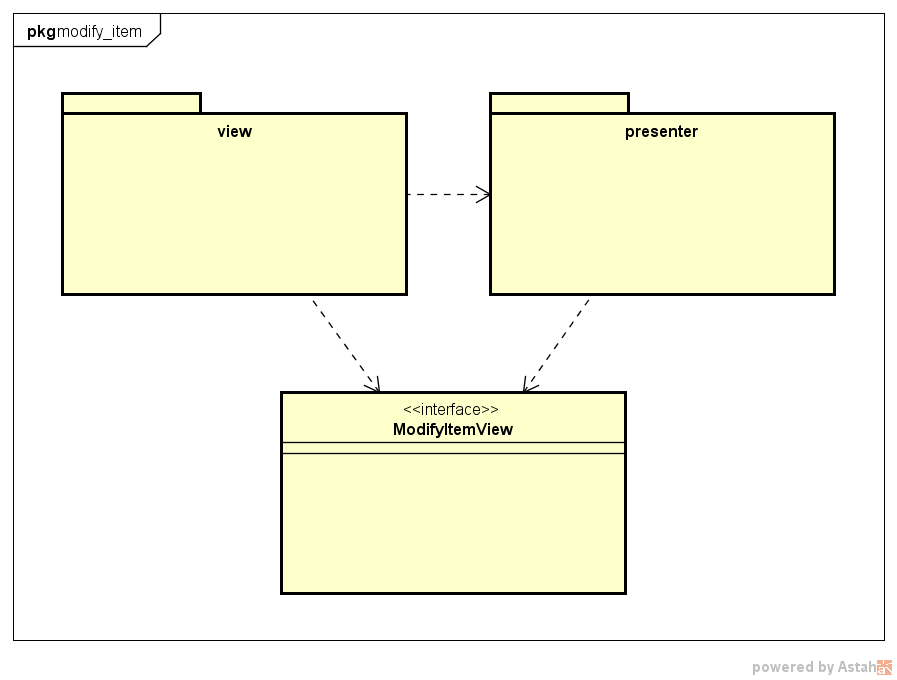
\includegraphics[scale=0.5]{Sezioni/Packages/App/modify_item.png}
	\caption{Package application::feature::modify\_item}
\end{figure}
\begin{itemize}
	\item \textbf{Descrizione}: package contenente i componenti per la funzionalità di modifica di un oggetto all'interno di una lista
	\item \textbf{Classi e packages contenuti}:
	\begin{itemize}
	\item application::feature::modify\_item::view: package contenente la vista per la modifica di un oggetto all'interno di una lista
	\item application::feature::modify\_item::presenter: package contenente il presenter per la vista di modifica di un oggetto all'interno di una lista
	\item application::feature::modify\_item::ModifyItemView: interfaccia rappresentante la vista per la funzionalità modifica di un oggetto all'interno di una lista
	\end{itemize}
\end{itemize}

\subsubsection{Package application::feature::modify\_item::view}
\label{Package application::feature::modify_item::view}
\begin{figure}[H]
	\centering
	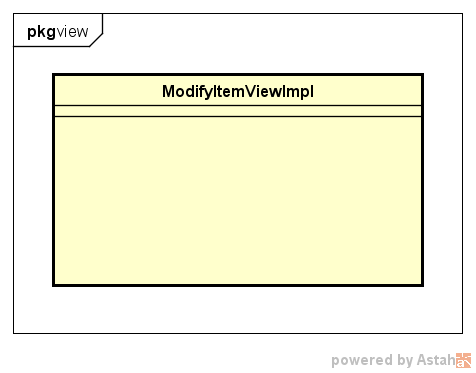
\includegraphics[scale=0.5]{Sezioni/Packages/App/modify_item_view.png}
	\caption{Package application::feature::modify\_item::view}
\end{figure}
\begin{itemize}
	\item \textbf{Descrizione}: package contenente la vista per la funzionalità di modifica di un oggetto all'interno di una lista
	\item \textbf{Classi e packages contenuti}:
	\begin{itemize}
	\item application::feature::modify\_item::view::ModifyItemViewImpl: implementazione dell'interfaccia che rappresenta la vista per la funzionalità di modifica di un oggetto all'interno di una lista
	\end{itemize}
\end{itemize}

\subsubsection{Package application::feature::modify\_item::presenter}
\label{Package application::feature::modify_item::presenter}
\begin{figure}[H]
	\centering
	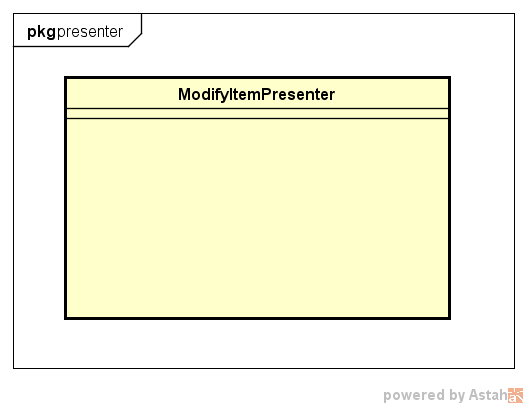
\includegraphics[scale=0.5]{Sezioni/Packages/App/modify_item_presenter.png}
	\caption{Package application::feature::modify\_item::presenter}
\end{figure}
\begin{itemize}
	\item \textbf{Descrizione}: package contenente il presenter per la vista di modifica di un oggetto all'interno di una lista
	\item \textbf{Classi e packages contenuti}:
	\begin{itemize}
	\item application::feature::modify\_item::presenter::ModifyItemViewPresenter: classe che rappresenta il presenter per la vista di modifica di un oggetto all'interno di una lista
	\end{itemize}
\end{itemize}


\subsubsection{Package application::feature::remove\_item}
\label{Package application::feature::remove_item}
\begin{figure}[H]
	\centering
	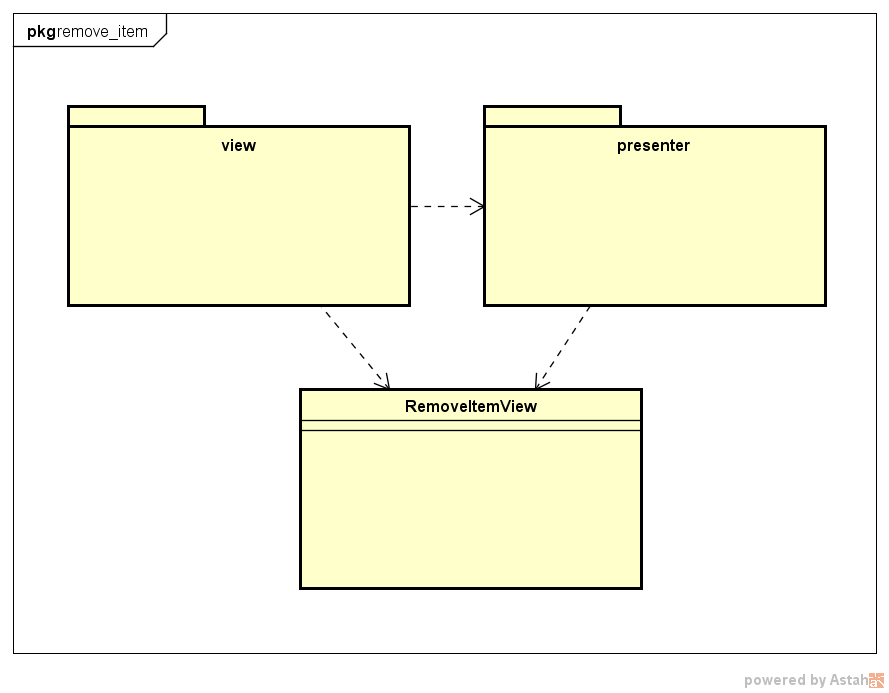
\includegraphics[scale=0.5]{Sezioni/Packages/App/remove_item.png}
	\caption{Package application::feature::remove\_item}
\end{figure}
\begin{itemize}
	\item \textbf{Descrizione}: package contenente i componenti per la funzionalità di rimozione di un oggetto da una lista
	\item \textbf{Classi e packages contenuti}:
	\begin{itemize}
	\item application::feature::remove\_item::view: package contenente la vista per la modifica di un oggetto all'interno di una lista
	\item application::feature::remove\_item::presenter: package contenente il presenter per la vista di modifica di un oggetto all'interno di una lista
	\item application::feature::remove\_item::RemoveItemView: interfaccia rappresentante la vista per la funzionalità modifica di un oggetto all'interno di una lista
	\end{itemize}
\end{itemize}

\subsubsection{Package application::feature::remove\_item::view}
\label{Package application::feature::remove_item::view}
\begin{figure}[H]
	\centering
	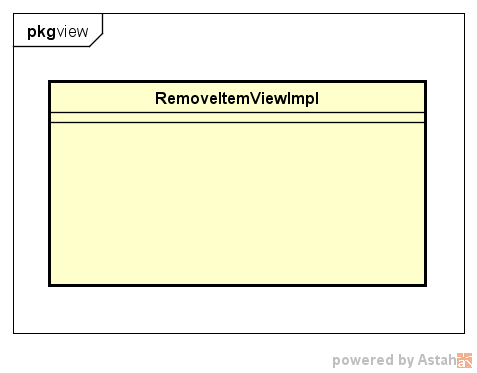
\includegraphics[scale=0.5]{Sezioni/Packages/App/remove_item_view.png}
	\caption{Package application::feature::remove\_item::view}
\end{figure}
\begin{itemize}
	\item \textbf{Descrizione}: package contenente la vista per la funzionalità di rimozione di un oggetto da una lista
	\item \textbf{Classi e packages contenuti}:
	\begin{itemize}
	\item application::feature::remove\_item::view::RemoveItemViewImpl: implementazione dell'interfaccia che rappresenta la vista per la funzionalità di rimozione di un oggetto da una lista
	\end{itemize}
\end{itemize}

\subsubsection{Package application::feature::remove\_item::presenter}
\label{Package application::feature::remove_item::presenter}
\begin{figure}[H]
	\centering
	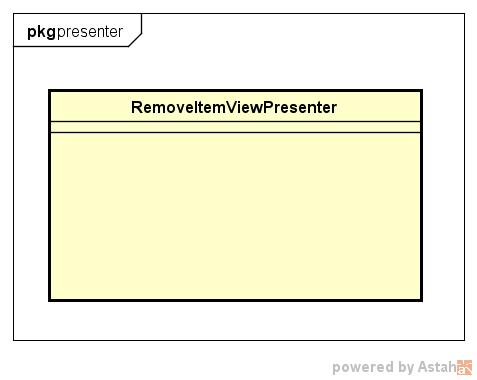
\includegraphics[scale=0.5]{Sezioni/Packages/App/remove_item_presenter.png}
	\caption{Package application::feature::forward::remove\_item::presenter}
\end{figure}
\begin{itemize}
	\item \textbf{Descrizione}: package contenente il presenter per la vista di rimozione di un oggetto da una lista
	\item \textbf{Classi e packages contenuti}:
	\begin{itemize}
	\item application::feature::remove\_item::presenter::RemoveItemViewPresenter: classe che rappresenta il presenter per la vista di rimozione di un oggetto da una lista
	\end{itemize}
\end{itemize}


\subsubsection{Package application::feature::sharewithcontact}
\label{Package application::feature::sharewithcontact}
\begin{figure}[H]
	\centering
	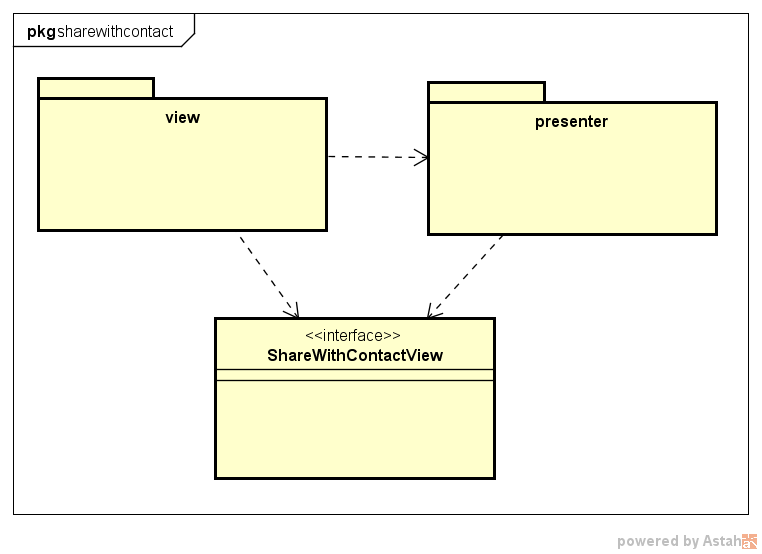
\includegraphics[scale=0.5]{Sezioni/Packages/App/share_with_contact.png}
	\caption{Package application::feature::sharewithcontact}
\end{figure}
\begin{itemize}
	\item \textbf{Descrizione}: package contenente i componenti per la funzionalità di condivisione della lista con un contatto
	\item \textbf{Classi e packages contenuti}:
	\begin{itemize}
	\item application::feature::sharewithcontact::view: package contenente la vista per la modifica di un oggetto all'interno di una lista
	\item application::feature::sharewithcontact::presenter: package contenente il presenter per la vista di modifica di un oggetto all'interno di una lista
	\item application::feature::sharewithcontact::ShareWithContactView: interfaccia rappresentante la vista per la funzionalità modifica di un oggetto all'interno di una lista
	\end{itemize}
\end{itemize}

\subsubsection{Package application::feature::sharewithcontact::view}\label{Package application::feature::sharewithcontact::view}
\begin{figure}[H]
	\centering
	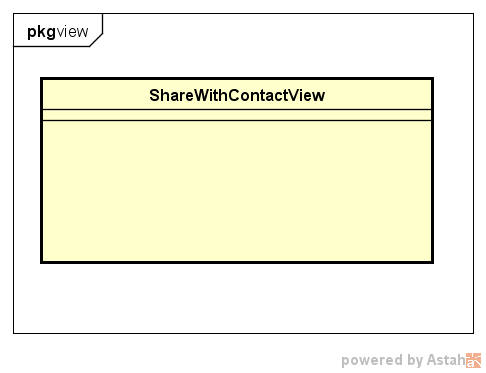
\includegraphics[scale=0.5]{Sezioni/Packages/App/share_with_contact_view.png}
	\caption{Package application::feature::sharewithcontact::view}
\end{figure}
\begin{itemize}
	\item \textbf{Descrizione}: package contenente la vista per la funzionalità di condivisione della lista con un contatto
	\item \textbf{Classi e packages contenuti}:
	\begin{itemize}
	\item application::feature::sharewithcontact::view::ShareWithContactViewImpl: implementazione dell'interfaccia che rappresenta la vista per la funzionalità di condivisione della lista con un contatto
	\end{itemize}
\end{itemize}

\subsubsection{Package application::feature::sharewithcontact::presenter}
\label{Package application::feature::sharewithcontact::presenter}
\begin{figure}[H]
	\centering
	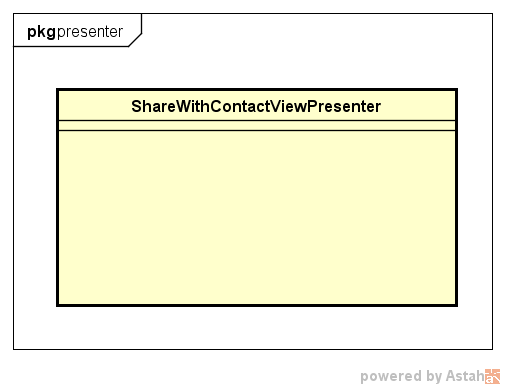
\includegraphics[scale=0.5]{Sezioni/Packages/App/share_with_contact_presenter.png}
	\caption{Package application::feature::sharewithcontact::presenter}
\end{figure}
\begin{itemize}
	\item \textbf{Descrizione}: package contenente il presenter per la vista di condivisione della lista con un contatto
	\item \textbf{Classi e packages contenuti}:
	\begin{itemize}
	\item application::feature::sharewithcontact::presenter::ShareWithContactViewPresenter: classe che rappresenta il presenter per la vista di condivisione della lista con un contatto
	\end{itemize}
\end{itemize}


\subsubsection{Package application::feature::sharewithgroup}
\label{Package application::feature::sharewithgroup}
\begin{figure}[H]
	\centering
	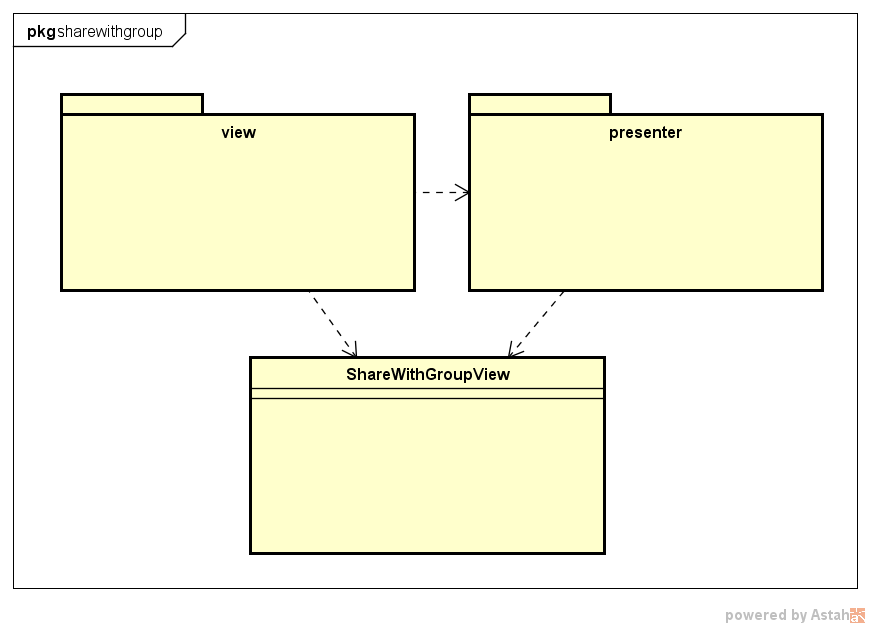
\includegraphics[scale=0.5]{Sezioni/Packages/App/share_with_group.png}
	\caption{Package application::feature::sharewithgroup}
\end{figure}
\begin{itemize}
	\item \textbf{Descrizione}: package contenente i componenti per la funzionalità di condivisione della lista con un gruppo
	\item \textbf{Classi e packages contenuti}:
	\begin{itemize}
	\item application::feature::sharewithgroup::view: package contenente la vista per la modifica di un oggetto all'interno di una lista
	\item application::feature::sharewithgroup::presenter: package contenente il presenter per la vista di modifica di un oggetto all'interno di una lista
	\item application::feature::sharewithgroup::ShareWithGroupView: interfaccia rappresentante la vista per la funzionalità modifica di un oggetto all'interno di una lista
	\end{itemize}
\end{itemize}

\subsubsection{Package application::feature::sharewithgroup::view}
\label{Package application::feature::sharewithgroup::view}
\begin{figure}[H]
	\centering
	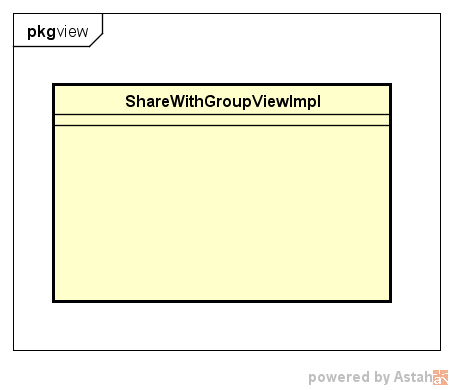
\includegraphics[scale=0.5]{Sezioni/Packages/App/share_with_group_view.png}
	\caption{Package application::feature::sharewithgroup::view}
\end{figure}
\begin{itemize}
	\item \textbf{Descrizione}: package contenente la vista per la funzionalità di condivisione della lista con un gruppo
	\item \textbf{Classi e packages contenuti}:
	\begin{itemize}
	\item application::feature::sharewithgroup::view::ShareWithGroupViewImpl: implementazione dell'interfaccia che rappresenta la vista per la funzionalità di condivisione della lista con un gruppo
	\end{itemize}
\end{itemize}

\subsubsection{Package application::feature::sharewithgroup::presenter}
\label{Package application::feature::sharewithgroup::presenter}
\begin{figure}[H]
	\centering
	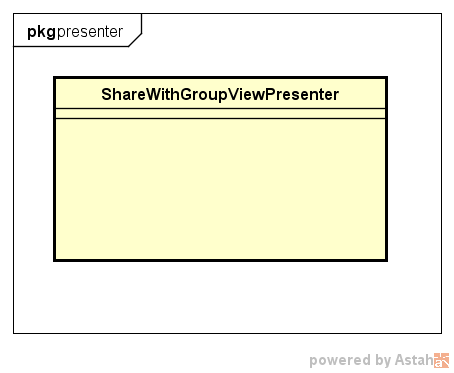
\includegraphics[scale=0.5]{Sezioni/Packages/App/share_with_group_presenter.png}
	\caption{Package application::feature::sharewithgroup::presenter}
\end{figure}
\begin{itemize}
	\item \textbf{Descrizione}: package contenente il presenter per la vista di condivisione della lista con un gruppo
	\item \textbf{Classi e packages contenuti}:
	\begin{itemize}
	\item application::feature::sharewithgroup::presenter::ShareWithGroupViewPresenter: classe che rappresenta il presenter per la vista di condivisione della lista con un gruppo
	\end{itemize}
\end{itemize}


\subsubsection{Package application::feature::help}
\label{Package application::feature::help}
\begin{figure}[H]
	\centering
	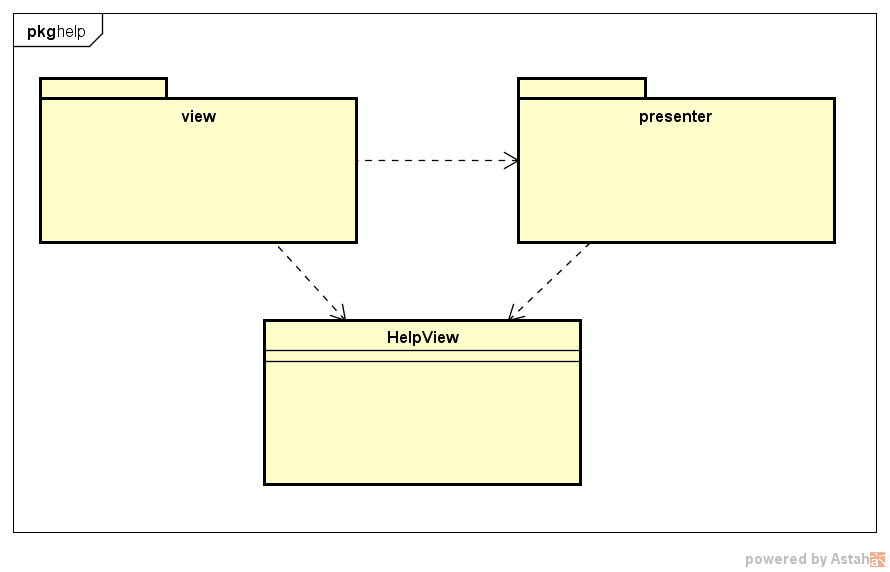
\includegraphics[scale=0.5]{Sezioni/Packages/App/help.png}
	\caption{Package application::feature::help}
\end{figure}
\begin{itemize}
	\item \textbf{Descrizione}: package contenente i componenti per la funzionalità di visualizzazione aiuto per l'utilizzo dell'applicazione
	\item \textbf{Classi e packages contenuti}:
	\begin{itemize}
	\item application::feature::help::view: package contenente la vista per la modifica di un oggetto all'interno di una lista
	\item application::feature::help::presenter: package contenente il presenter per la vista di modifica di un oggetto all'interno di una lista
	\item application::feature::help::helpView: interfaccia rappresentante la vista per la funzionalità modifica di un oggetto all'interno di una lista
	\end{itemize}
\end{itemize}

\subsubsection{Package application::feature::help::view}
\label{Package application::feature::help::view}
\begin{figure}[H]
	\centering
	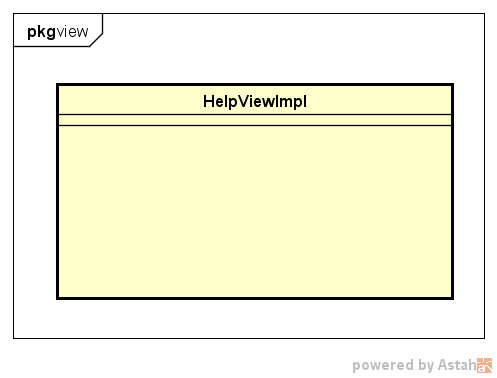
\includegraphics[scale=0.5]{Sezioni/Packages/App/help_view.png}
	\caption{Package application::feature::help::view}
\end{figure}
\begin{itemize}
	\item \textbf{Descrizione}: package contenente la vista per la funzionalità di visualizzazione aiuto per l'utilizzo dell'applicazione
	\item \textbf{Classi e packages contenuti}:
	\begin{itemize}
	\item application::feature::help::view::helpViewImpl: implementazione dell'interfaccia che rappresenta la vista per la funzionalità di visualizzazione aiuto per l'utilizzo dell'applicazione
	\end{itemize}
\end{itemize}

\subsubsection{Package application::feature::help::presenter}
\label{Package application::feature::help::presenter}
\begin{figure}[H]
	\centering
	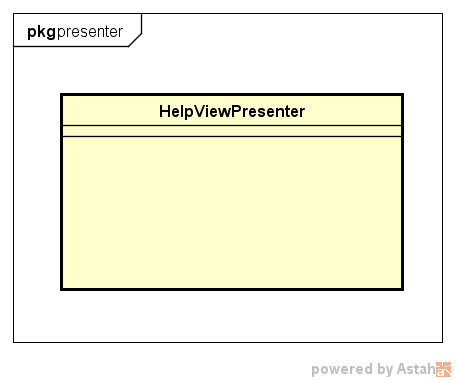
\includegraphics[scale=0.5]{Sezioni/Packages/App/help_presenter.png}
	\caption{Package application::feature::help::presenter}
\end{figure}
\begin{itemize}
	\item \textbf{Descrizione}: package contenente il presenter per la vista di visualizzazione aiuto per l'utilizzo dell'applicazione
	\item \textbf{Classi e packages contenuti}:
	\begin{itemize}
	\item application::feature::help::presenter::helpViewPresenter: classe che rappresenta il presenter per la vista di visualizzazione aiuto per l'utilizzo dell'applicazione
	\end{itemize}
\end{itemize}

\subsubsection{Package application::feature::exception}
\label{Package application::feature::exception}
\begin{figure}[H]
	\centering
	\includegraphics[scale=0.5]{Sezioni/Packages/App/exception.png}
	\caption{Package application::feature::exception}
\end{figure}
\begin{itemize}
	\item \textbf{Descrizione}: package contenente tutte le eccezioni che l'applicazione può lanciare durante l'esecuzione
	\item \textbf{Classi e packages contenuti}:
	\begin{itemize}
	\item application::feature::exception::Exception: classe che rappresenta una eccezione generica
	\item application::feature::exception::BadParameterException: classe che rappresenta una eccezione lanciata nel qual caso un parametro di un metodo sia incorretto
	\end{itemize}
\end{itemize}


\newpage